\chapter{Méthode CREA : \MyCREA}
\label{chapter:CREA}

Dans ce chapitre, nous détaillons la méthode CREA en trois sections.
Tout d'abord, une présentation générale de la méthode est faite pour expliquer les objectifs visés, le cadre général de travail qui a été utilisé lors de la conception, et le fonctionnement global de la méthode.
Les deux sections suivantes traitent plus en détails des phases de pré-traitement sémantique, visant à extraire les termes représentant les connaissances réutilisables des documents d'entrée, et d'analyse structurelle qui génère les regroupements  de termes représentants la structure, ainsi que des métriques concernant les termes et documents d'entrée.

\bigskip

\minitoc % Creating an actual minitoc / ToC local to a chapter

\newpage

%%%%%%%%%%%%%%%%%%%%%%%%%%%%%%%%%%%%%%%%%%%%%%%%%%%%%%%%%%%%%%%%

\section{Présentation générale de la méthode et cadre de travail}
\label{section:CREA:PresentationGenerale}

\subsection{Objectifs de la méthode}
\label{subsection:CREA:ObjectifsMethode}

%%% POURQUOI

La méthode CREA, ou \textit{\MyCREA}, vise à répondre à plusieurs défis exposés en section~\ref{subsubsection:Contexte:KIP-RevueLitterature:KIP:DifficulteGestionKIP}, en particulier la réutilisation de fragments issus de cas passés pour former des nouveaux cours, et la prise en compte du contexte au travers de la vérification de la pertinence des documents.
Dans les travaux de cette thèse, les cas passés correspondent aux cours (et les supports associés) générés par d'autres enseignants, voire tous les documents actuellement disponibles traitant du sujet (articles de recherche, présentation technique, etc).
Les fragments réutilisables correspondent aux notions abordées dans les cours.
Précisément, il s'agit des termes associés à ces notions regroupés sous forme de clusters.
Un utilisateur souhaitant traiter un nouveau cas se verra proposer des fragments issus de plusieurs documents générés lors d'exécutions de précédents cas grâce à la méthode CREA.
Ces fragments lui permettent d'adapter ses décisions en se basant sur des données qui ont été générées lors de cas passés qu'il a sélectionnés.
Ces cas passés ont été gérés par d'autres utilisateurs qui leur ont associé des données en s'appuyant sur leur propre expertise (ou connaissances tacites).

L'objectif de la méthode CREA est donc de profiter de ces expériences passées pour proposer les meilleurs regroupements (ou \textit{clusters}) de données aptes à répondre au nouveau cas, le tout de façon la plus automatisée possible.
La construction d'un nouveau cas, et l'évaluation de sa pertinence par rapport au sujet traité, s'effectuent en analysant les notions présentes dans les documents au travers des termes les constituant.
Des métriques permettent d'illustrer l'absence ou la présence de termes dans les documents et les écarts entre documents.
Ainsi, il est possible d'aider l'utilisateur à améliorer la qualité des regroupements en exploitant une des métriques pour conserver (ou supprimer) des documents ou des termes.
Un second usage de cette métrique permet également d'évaluer la pertinence de son propre support de cours en le comparant à de nombreux autres.

\bigskip

Dans le domaine de l'enseignement supérieur et de la recherche, la méthode CREA permet de générer automatiquement à partir de supports de cours existants un syllabus de cours découpé en autant de séances que l'enseignant souhaite.
Des documents de nature plus variée, tels que des articles de recherche ou des présentations techniques, peuvent y être adjoints.
Un enseignant souhaitant construire un nouveau cours doit uniquement fournir en entrée de la méthode CREA le nombre de séances visées et des supports de cours existant, afin de pouvoir obtenir une proposition de structure de syllabus en sortie.
Précisément, les notions essentielles des supports de cours sont extraites, analysées, puis ré-assemblées sous formes de clusters pour pouvoir les proposer à l'enseignant.
Le nombre de clusters fourni est égal au nombre de séances demandées par l'enseignant.
L'évaluation de la pertinence des supports de cours fournis par l'enseignant est possible grâce à une métrique explicitant quelles notions centrales sont partagées par tous les documents, ou éventuellement quels supports sont éloignés, voire sont hors sujet.
L'ordonnancement des clusters formant la structure du syllabus est encore en cours d'évaluation, elle est néanmoins discutée en section~\ref{subsection:Conclusion:PerspectivesAmeliorations:AnalyseTemporelle} afin de montrer tout le potentiel de la méthode CREA.



\subsection{Cadre de travail}
\label{subsection:CREA:CadreTravail}

%%% QUOI

La réutilisation de fragments issus de cas passés implique de se positionner selon le point de vue de la gestion de cas, et non pas seulement des processus à forte intensité de connaissances : chaque cas est unique, bien que des similitudes puissent exister.
L'autre intérêt de ce point de vue est qu'il est dirigé par les données, ce qui permet de se concentrer sur celles-ci pour pouvoir exposer les meilleures informations aux utilisateurs impliqués et les aider à prendre les meilleures décisions.
Le traitement d'un cas, jusqu'à sa résolution, produit donc des données réutilisables par la suite.

\bigskip

Dans le cadre de l'enseignement supérieur, les enseignants sont considérés comme les utilisateurs.
Chaque enseignant a sa propre expertise qui diffère d'un individu à l'autre, qu'ils aient suivi le même parcours ou non.
Les cas étudiés concernent les cours universitaires, et particulièrement l'aide à la construction de supports de cours.
Chaque cas traité (instance de processus) produit donc un support de cours (les données du cas) dont les fragments réutilisables correspondent aux notions sélectionnées par l'enseignant.
Ces supports de cours générés consolident donc l'ensemble des notions à aborder en cours magistral, en travaux dirigés, voire en travaux pratiques.
Bien que ces supports de cours puissent être constitués d'images, sons, vidéos ou de nombreux autres médias variés, nous nous concentrons exclusivement sur les cours dont le contenu est majoritairement constitué de texte.
Ces textes peuvent facilement être traités automatiquement et découpés en termes dont le ré-agencement permet de construire des clusters rassemblant plusieurs notions à enseigner.
Ces clusters de termes permettent directement de proposer une structure de syllabus qu'un enseignant peut réutiliser partiellement ou complètement lorsqu'il construit un nouveau cours.
Les niveaux de granularité retenus des données traitées correspondent aux supports de cours texte contenant des notions à aborder, dont les termes sont manipulés (sélectionnés, filtrés, standardisés, ...) pour former des clusters assimilables à la structure d'un syllabus de cours.



\subsection{Fonctionnement général}
\label{subsection:CREA:FonctionnementGeneralSemantique}

%%% COMMENT

La méthode CREA se divise actuellement en deux phases principales de pré-traitement sémantique (PI) puis d'analyse structurelle (PII), comme illustré sur la figure~\ref{figure:3-MethodeGenerale}.
Une troisième phase d'analyse temporelle est encore en cours d'évaluation et est présentée en section~\ref{subsection:Conclusion:PerspectivesAmeliorations:AnalyseTemporelle}.
L'atout majeur de CREA réside dans l'automatisation complète de chacune des phases la composant, bien qu'il soit possible de paramétrer plus finement certaines étapes pour améliorer la qualité des résultats.
La phase de pré-traitement sémantique (PI) vise à extraire les termes des documents donnés en entrée, tandis que la phase d'analyse structurelle (PII) expose tout d'abord des métriques sur la pertinence des documents entre eux (l'impact mutuel présenté en sous-section~\ref{mystep:Contexte:ACF-MetriquesTreillis-ImpactMutuel}), puis construit les clusters de termes explicitant la structure des documents fournis afin de pouvoir les réutiliser.


%\begin{figure*} % Figure flottante
\begin{figure}[ht]
\centering
%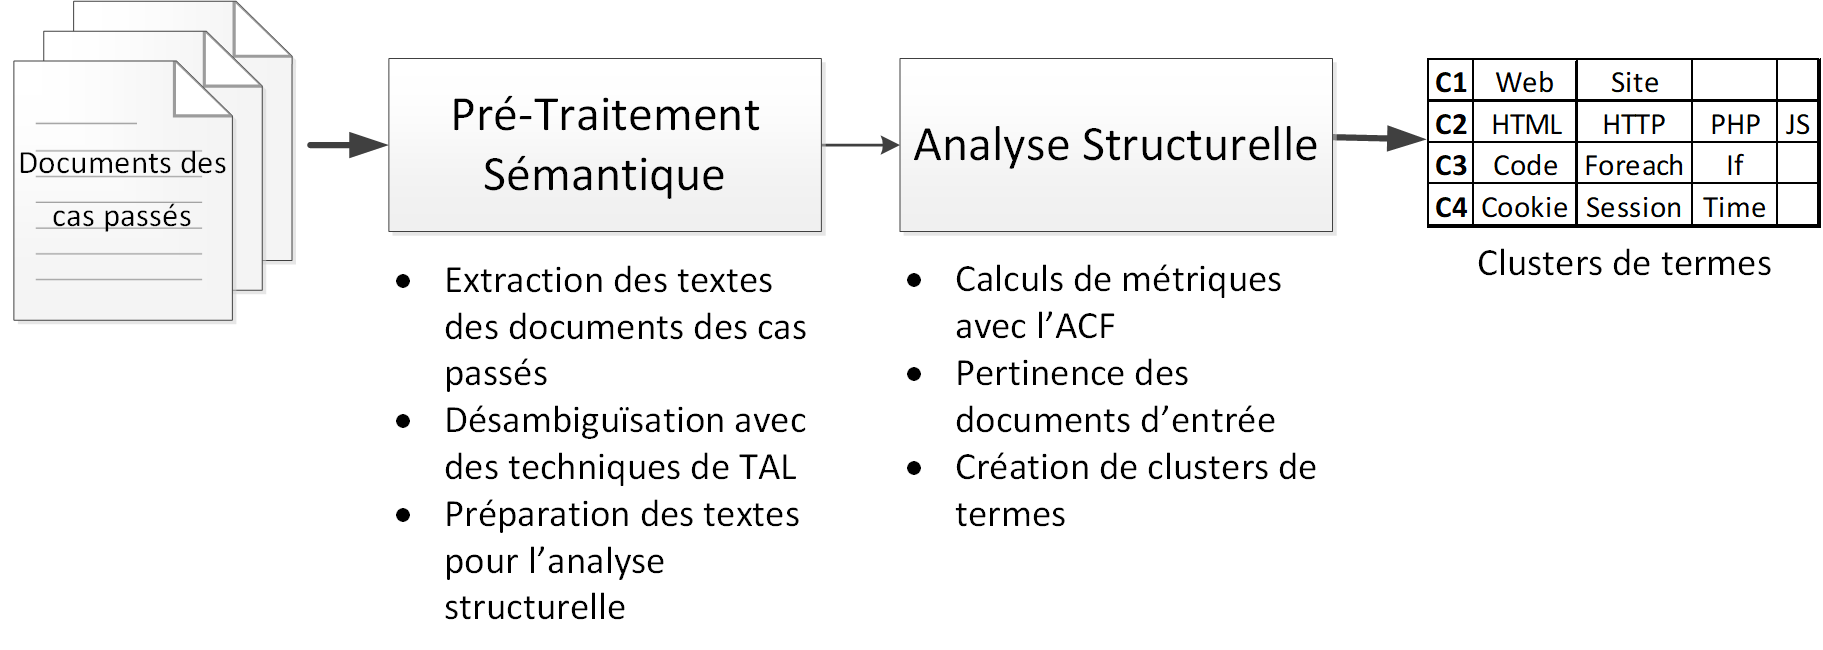
\includegraphics[width=3in]{3-Methode-CREA/images/schema_general.png}
\centerline{  % FORCE FIGURE OUTSIDE THE MARGIN !!! BUT STILL CENTERING !!!
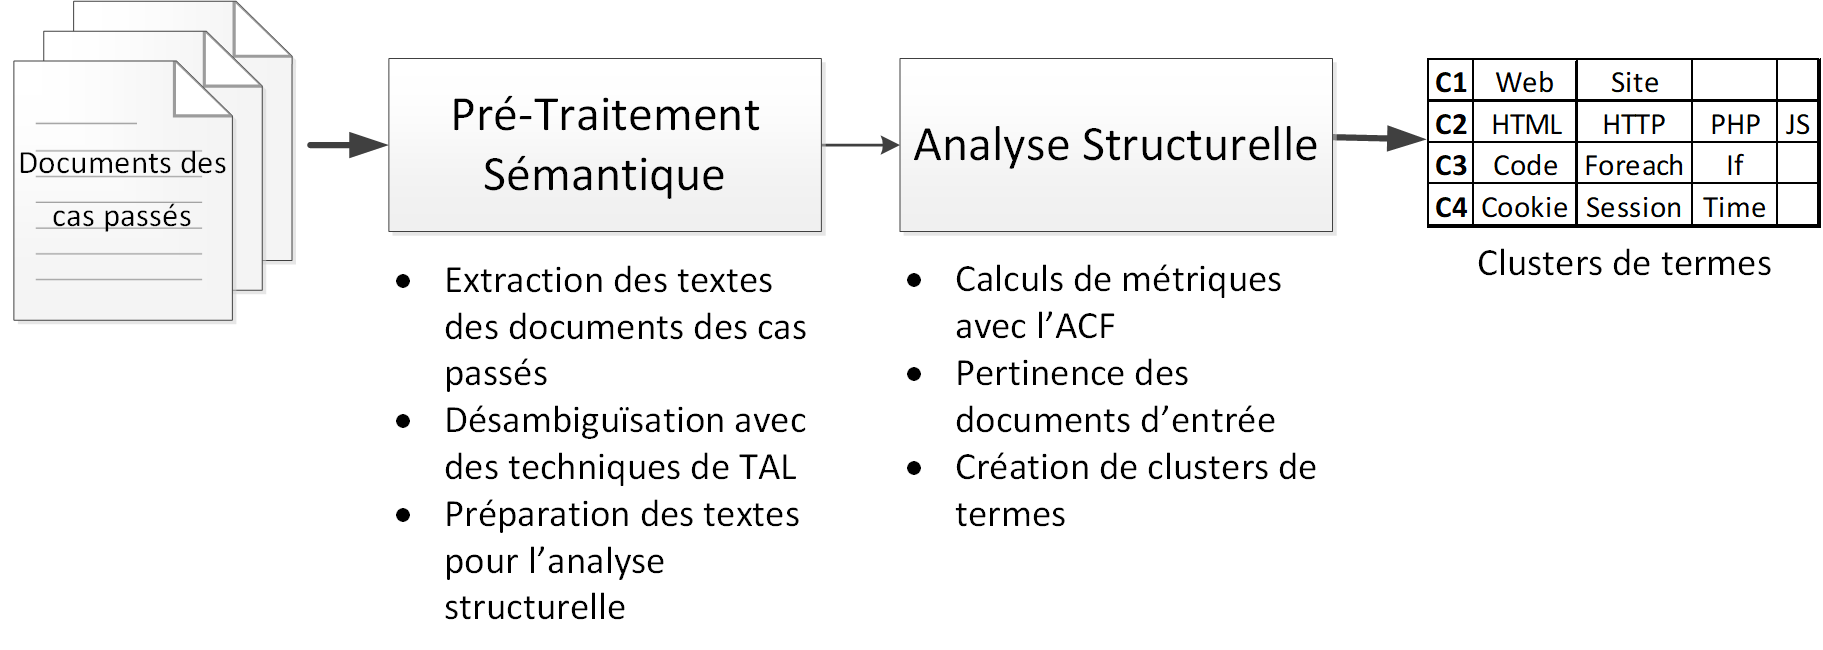
\includegraphics[scale=0.7]{3-Methode-CREA/images/schema_general.png}
}
\caption{Les deux principales phases de la méthode CREA}
\label{figure:3-MethodeGenerale}
\end{figure}
%\end{figure*} % Figure flottante
% To use it : fig~\ref{label}

\bigskip

La phase de pré-traitement sémantique (PI) est divisée en cinq étapes qui s'appuient sur plusieurs techniques de traitement automatique du langage présentées en section~\ref{subsection:Contexte:TechniquesUtilisees:TAL}.
Ces étapes permettent d'extraire les termes des documents sélectionnés, puis de lier ces termes à des entités reconnues dans des bases de connaissances grâce à une étape de désambiguïsation.
Ces bases de connaissances permettent de standardiser les entités manipulées dans l'ensemble du corpus de textes en faisant abstraction des synonymes mais également des langues utilisées dans les documents.
À l'issue de ces cinq étapes, une liste de termes standardisés est générée pour chacun des documents.
Les traitements suivants s'appuient soit sur ce format en \textit{liste}, soit sur un format en \textit{matrice d'occurrences} de termes dans des documents comme illustré sur la figure~\ref{figure:3-MethodeGenerale-PI-outputs}.
Appliqué au cas de l'enseignement il s'agit donc de générer, pour chacun des supports de cours sélectionnés, une liste de termes standardisés et reconnus dans des bases de connaissances représentant les notions abordées dans le cours.


%\begin{figure*} % Figure flottante
\begin{figure}[ht]
\centering
\centerline{  % FORCE FIGURE OUTSIDE THE MARGIN !!! BUT STILL CENTERING !!!
% scale = 0.6   1 OK dans certaines circonstances
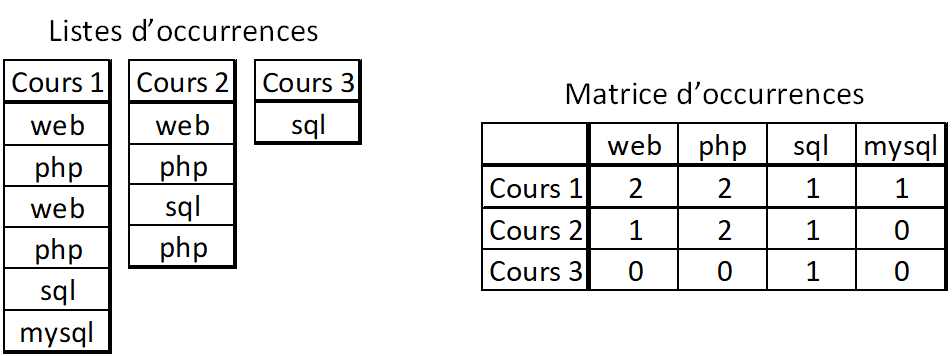
\includegraphics[scale=0.85]{3-Methode-CREA/images/0-fonctionnement-general/listes-et-matrice.png}
}
\caption{Exemple de listes et de matrice d'occurrences de termes générées à l'issue de la phase de pré-traitement sémantique (PI)}
\label{figure:3-MethodeGenerale-PI-outputs}
\end{figure}
%\end{figure*} % Figure flottante
% To use it : fig~\ref{label}

\bigskip

La phase d'analyse structurelle (PII) est divisée en trois grandes étapes qui s'appuient sur l'analyse de concepts formels, présentée en section~\ref{subsection:Contexte:TechniquesUtilisees:ACF}, et les méthodes de clustering, présentées en section~\ref{subsection:Contexte:TechniquesUtilisees:Clustering}.
Ces étapes permettent d'analyser les documents et les termes les composant, afin d'évaluer leur pertinence et d'en extraire les regroupements de termes les plus utiles à l'utilisateur.
Dans le domaine de l'enseignement, il s'agit donc de générer des métriques évaluant la qualité de la composition des supports de cours entre eux, afin de permettre à l'enseignant de supprimer des supports qui ne conviennent pas à ses exigences ou éventuellement des notions qu'il ne souhaite pas aborder, et pouvoir en extraire des clusters de termes représentant une structure de cours réutilisable.
Par exemple, si un enseignant souhaite construire un cours de développement web à l'aide de PHP en s'appuyant sur une dizaine de supports de cours, mais dont l'un traite en fait de Java, un graphique lui permettra de constater qu'un des supports de cours insérés est hors sujet et doit être vérifié pour éventuellement le retirer.
La figure~\ref{figure:3-MethodeGenerale-PII-output-graphe} montre que les supports C6 et CJA sont beaucoup plus éloignés des autres, et devraient être vérifiés manuellement.
Ensuite, lorsque le corpus de documents est considéré par l'enseignant comme convenable, des clusters peuvent être générés selon le nombre de séances souhaité.
La figure~\ref{figure:3-MethodeGenerale-PII-output-clusters} montre huit clusters générés à partir de plusieurs supports de cours de PHP (les clusters ne sont pas ordonnés), l'enseignant peut ainsi s'appuyer dessus pour préparer ses huit séances de cours.

%\begin{figure*} % Figure flottante
\begin{figure}[ht]
\centering
\centerline{  % FORCE FIGURE OUTSIDE THE MARGIN !!! BUT STILL CENTERING !!!
% scale = 0.6
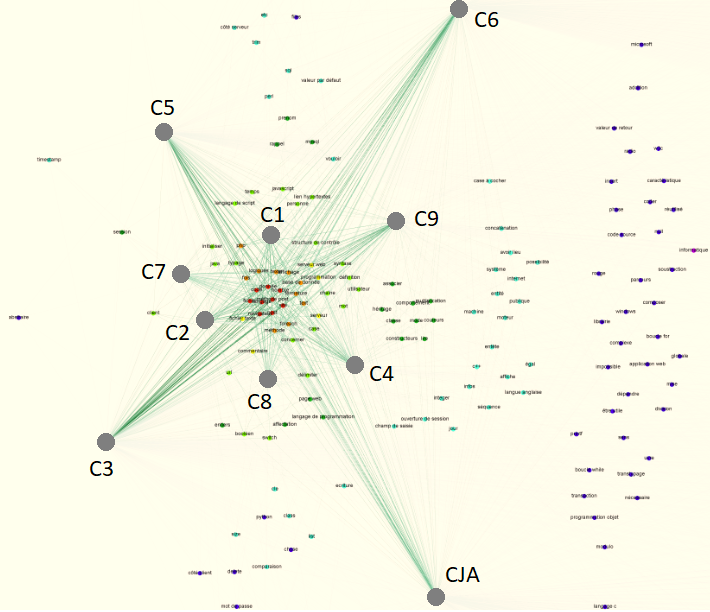
\includegraphics[scale=0.45]{3-Methode-CREA/images/0-fonctionnement-general/graphe-impact-mutuel.png}
}
\caption{Exemple de graphe d'impact mutuel explicitant que les supports C6 et CJA sont éloignés des autres}
\label{figure:3-MethodeGenerale-PII-output-graphe}
\end{figure}
%\end{figure*} % Figure flottante
% To use it : fig~\ref{label}

%\begin{figure*} % Figure flottante
\begin{figure}[ht]
\centering
\centerline{  % FORCE FIGURE OUTSIDE THE MARGIN !!! BUT STILL CENTERING !!!
% scale = 0.6
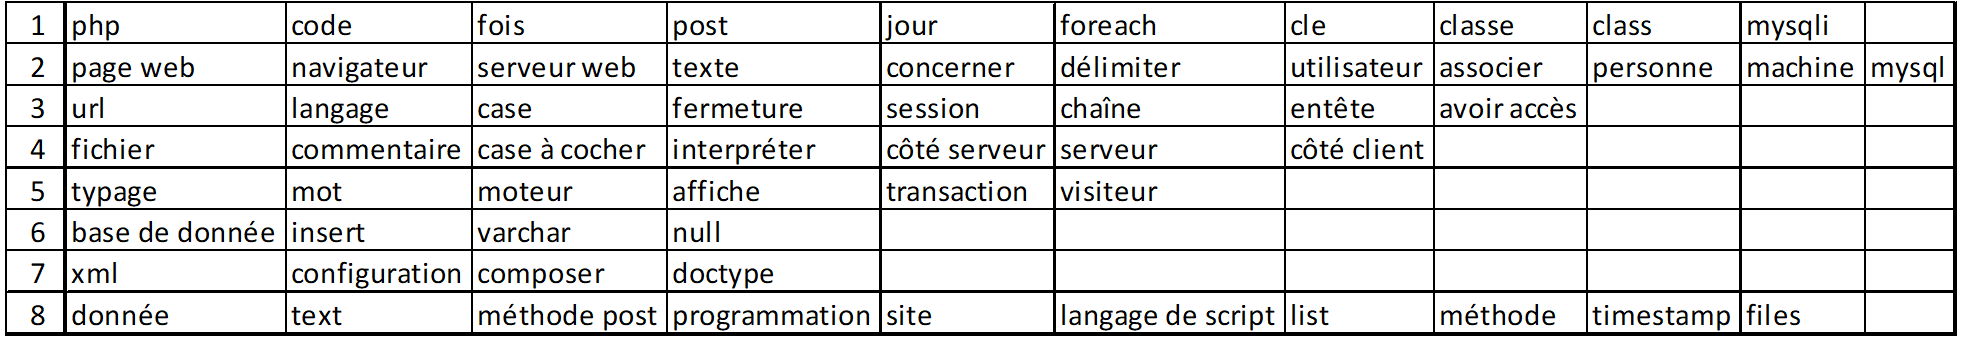
\includegraphics[scale=0.65]{3-Methode-CREA/images/0-fonctionnement-general/8-clusters.png}
}
\caption{Exemple de huit clusters générés avec la méthode CREA pour huit séances à partir de supports de cours sur PHP}
\label{figure:3-MethodeGenerale-PII-output-clusters}
\end{figure}
%\end{figure*} % Figure flottante
% To use it : fig~\ref{label}

\bigskip

La figure~\ref{figure:3-MethodeGeneraleFinale} explicite les étapes des deux phases tout en indiquant les données générées au fur et à mesure.
Comme indiqué précédemment, on observe que la première phase se concentre explicitement sur la préparation des documents fournis en entrée, afin de produire une matrice représentant l'ensemble des documents sélectionnés et les termes les composants.
La deuxième phase analyse en profondeur cette matrice pour en extraire des métriques qui servent à aider l'utilisateur à comprendre les données qu'il manipule et améliorer la qualité de sa base documentaires, le tout pour générer une structure réutilisable issue d'une liste de clusters de termes résumant ces documents.


%\begin{figure*} % Figure flottante
\begin{figure}[ht!]
\centering
%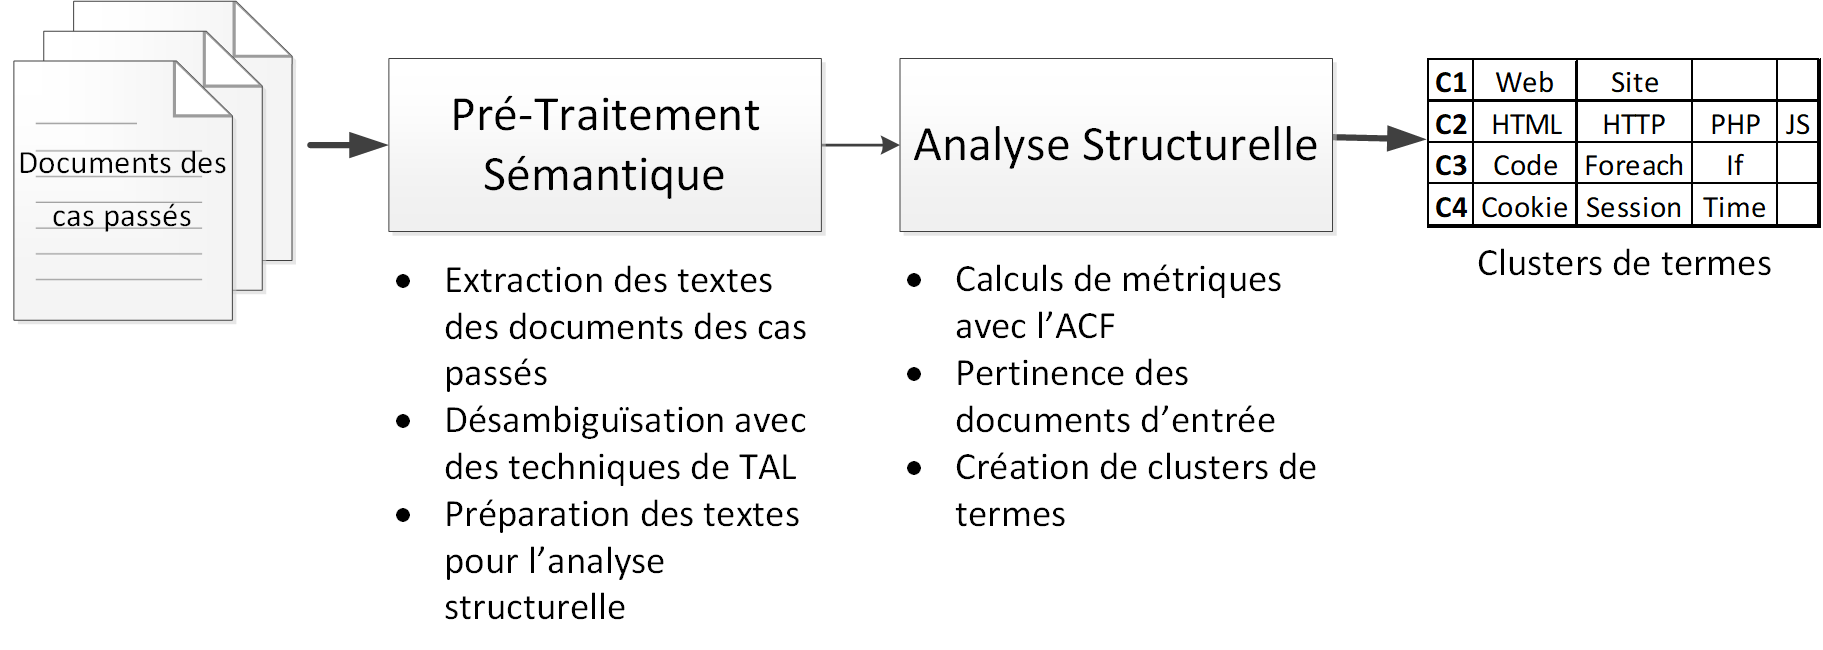
\includegraphics[width=3in]{3-Methode-CREA/images/schema_general.png}
\centerline{  % FORCE FIGURE OUTSIDE THE MARGIN !!! BUT STILL CENTERING !!!
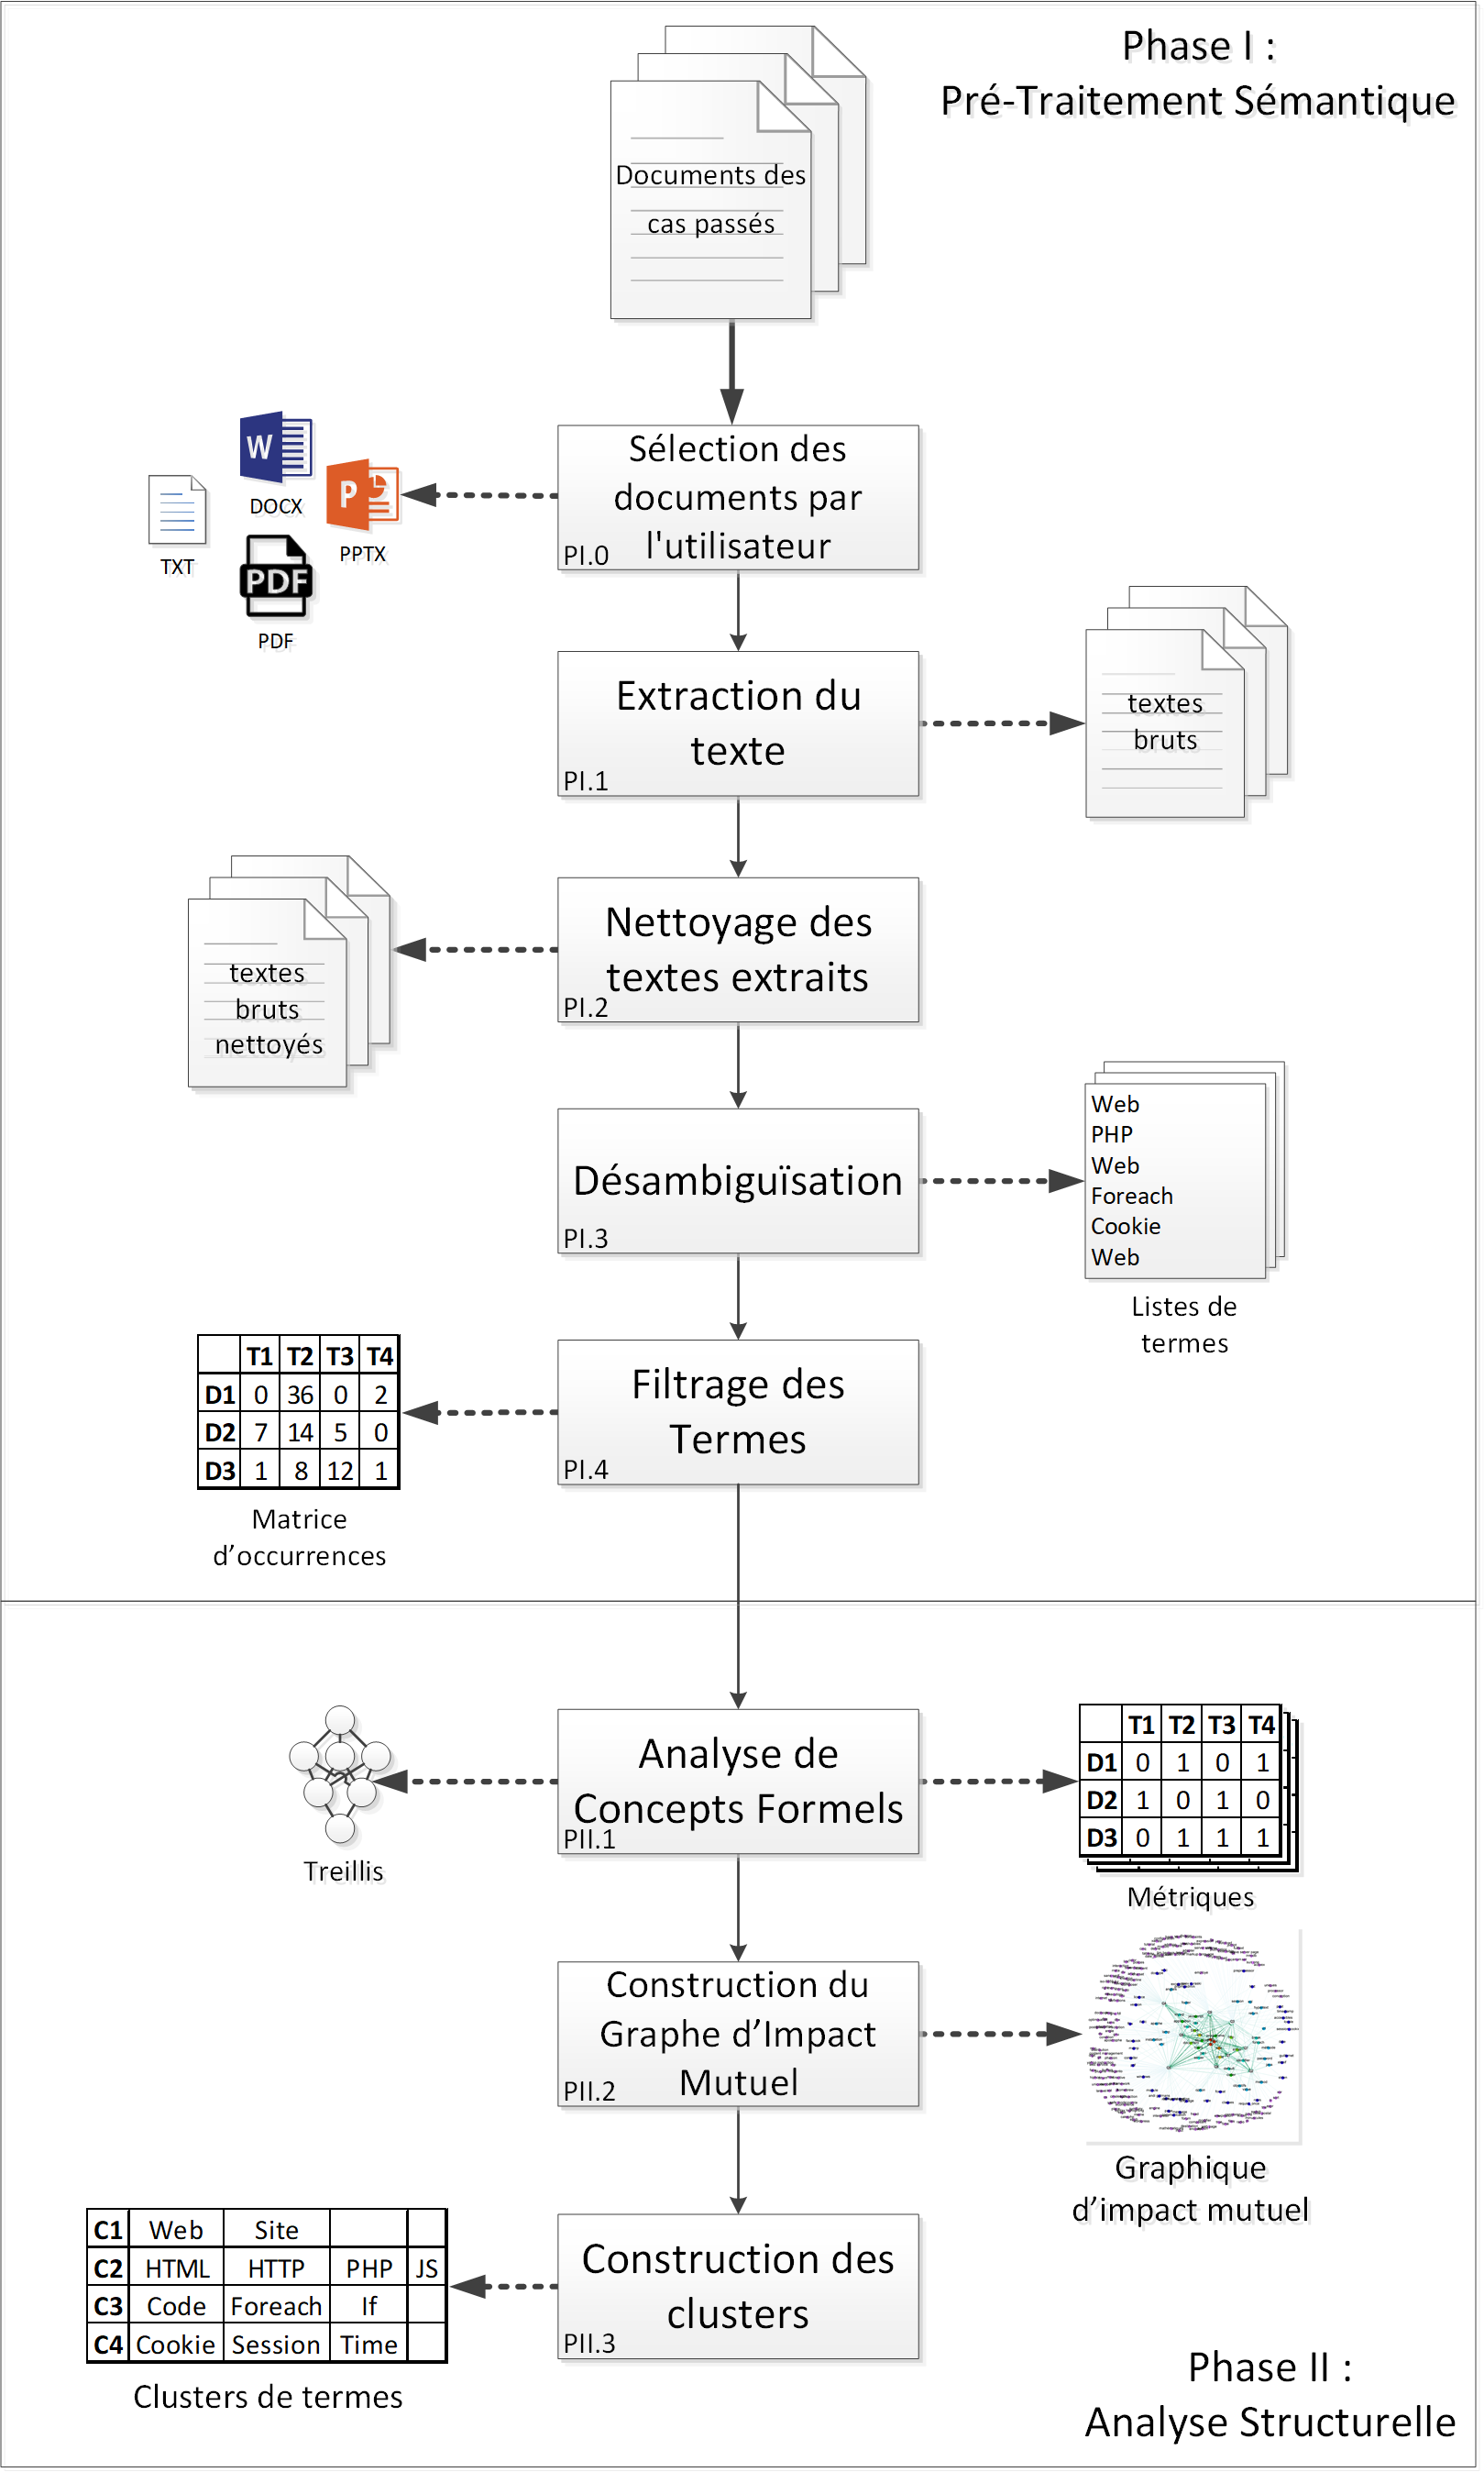
\includegraphics[scale=0.6]{3-Methode-CREA/images/schema_final.png}
}
\caption{Les deux phases détaillées de la méthode CREA}
\label{figure:3-MethodeGeneraleFinale}
\end{figure}
%\end{figure*} % Figure flottante
% To use it : fig~\ref{label}



%%%%%%%%%%%%%%%%%%%%%%%%%%%%%%%%%%%%%%%%%%%%%%%%%%%%%%%%%%%%%%%%%%%%%%%%%%%%%%%%%%%%%%%%%%
%%%%%%%%%%%%%%%%%%%%%%%%%%%%%%%%%%%%%%%%%%%%%%%%%%%%%%%%%%%%%%%%%%%%%%%%%%%%%%%%%%%%%%%%%%
%%%%%%%%%%%%%%%%%%%%%%%%%%%%%%%%%%%%%%%%%%%%%%%%%%%%%%%%%%%%%%%%%%%%%%%%%%%%%%%%%%%%%%%%%%
%%%%%%%%%%%%%%%%%%%%%%%%%%%%%%%%%%%%%%%%%%%%%%%%%%%%%%%%%%%%%%%%%%%%%%%%%%%%%%%%%%%%%%%%%%
%%%%%%%%%%%%%%%%%%%%%%%%%%%%%%%%%%%%%%%%%%%%%%%%%%%%%%%%%%%%%%%%%%%%%%%%%%%%%%%%%%%%%%%%%%
%%%%%%%%%%%%%%%%%%%%%%%%%%%%%%%%%%%%%%%%%%%%%%%%%%%%%%%%%%%%%%%%%%%%%%%%%%%%%%%%%%%%%%%%%%

%%%%%%%%%%%%%%%%%%%%%%%%%%%%%%%%%%%%%%%%%%%%
\clearpage % Clean for pictures and tables %
\newpage   % Clean for pictures and tables %
%%%%%%%%%%%%%%%%%%%%%%%%%%%%%%%%%%%%%%%%%%%%

%%%%%%%%%%%%%%%%%%%%%%%%%%%%%%%%%%%%%%%%%%%%%%%%%%%%%%%%%%%%%%%%%%%%%%%%%%%%%%%%%%%%%%%%%%
%%%%%%%%%%%%%%%%%%%%%%%%%%%%%%%%%%%%%%%%%%%%%%%%%%%%%%%%%%%%%%%%%%%%%%%%%%%%%%%%%%%%%%%%%%
%%%%%%%%%%%%%%%%%%%%%%%%%%%%%%%%%%%%%%%%%%%%%%%%%%%%%%%%%%%%%%%%%%%%%%%%%%%%%%%%%%%%%%%%%%
%%%%%%%%%%%%%%%%%%%%%%%%%%%%%%%%%%%%%%%%%%%%%%%%%%%%%%%%%%%%%%%%%%%%%%%%%%%%%%%%%%%%%%%%%%
%%%%%%%%%%%%%%%%%%%%%%%%%%%%%%%%%%%%%%%%%%%%%%%%%%%%%%%%%%%%%%%%%%%%%%%%%%%%%%%%%%%%%%%%%%
%%%%%%%%%%%%%%%%%%%%%%%%%%%%%%%%%%%%%%%%%%%%%%%%%%%%%%%%%%%%%%%%%%%%%%%%%%%%%%%%%%%%%%%%%%

\section{Pré-traitement sémantique : extraction des termes}
\label{section:CREA:PI-AnalyseSemantique}

La première phase (PI) de la méthode CREA, le pré-traitement sémantique, a pour objectif d'extraire une liste de termes à partir de documents fournis en entrée, et de les rassembler sous forme d'une matrice d'occurrences afin de les organiser plus tard sous forme de clusters.
Dans le contexte de l'enseignement supérieur, ces termes représentent les notions abordées dans les supports de cours fournis en entrée.
Cette première phase se déroule en cinq étapes successives illustrées par la figure~\ref{figure:3-I-PreTraitementSemantique}.

%\begin{figure*} % Figure flottante
\begin{figure}[ht]
\centering
\centerline{  % FORCE FIGURE OUTSIDE THE MARGIN !!! BUT STILL CENTERING !!!
% 0.49
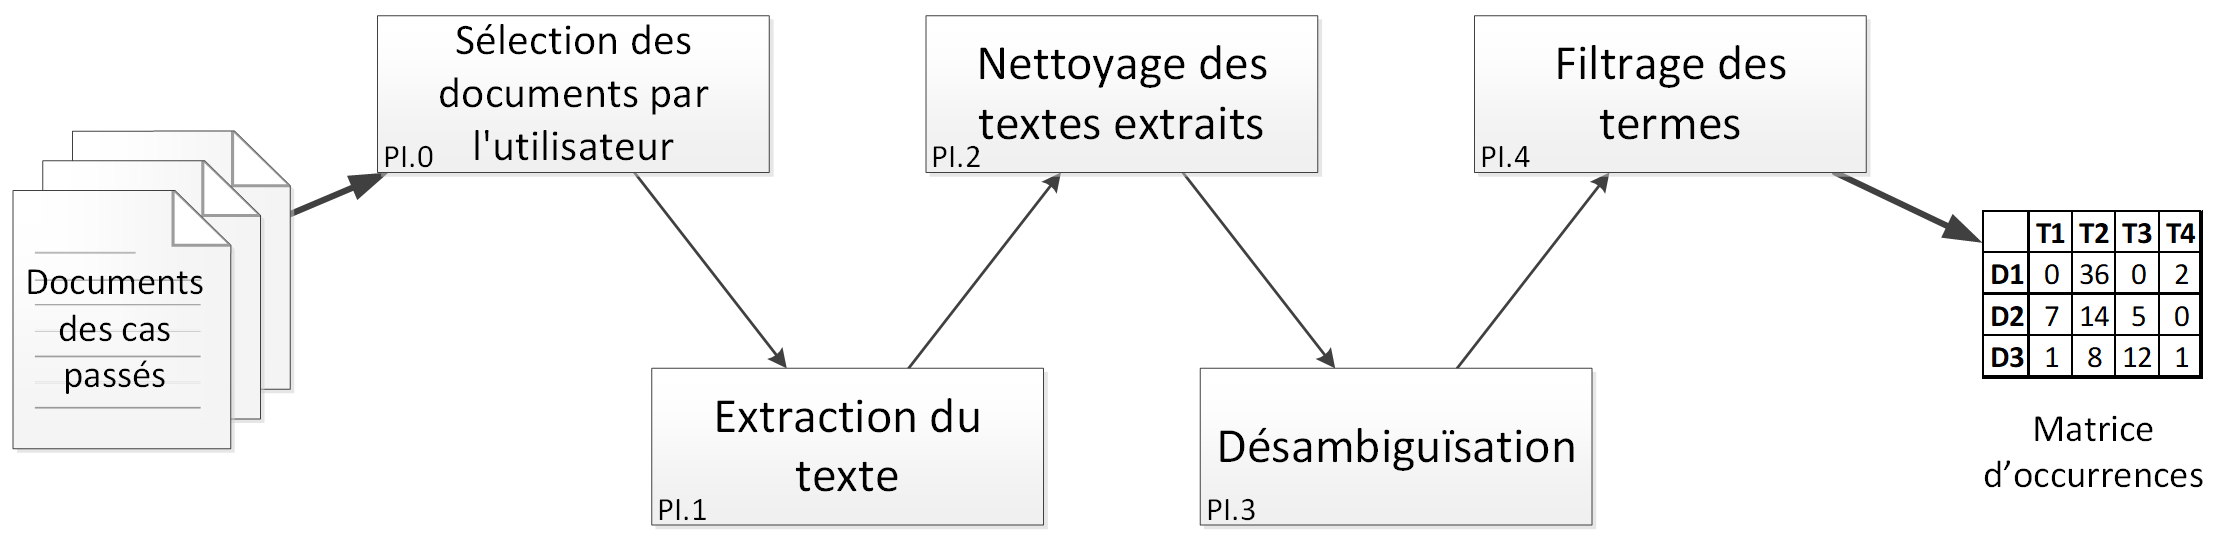
\includegraphics[scale=0.55]{3-Methode-CREA/images/schema_pre-traitement_semantique_ESCALIER.png}
}
\caption{Les étapes de la phase de pré-traitement sémantique}
\label{figure:3-I-PreTraitementSemantique}
\end{figure}
%\end{figure*} % Figure flottante
% To use it : fig~\ref{label}

\begin{itemize}
\item Sélection des documents par l'utilisateur (PI.0) : Tout d'abord, l'enseignant sélectionne des supports de cours dont les titres lui semblent pertinents et dont le contenu est majoritairement composé de texte.
\item Extraction du texte (PI.1) : Une étape d'extraction du texte s'appuie sur la reconnaissance optique de caractères (ou \textit{OCR}) pour pouvoir transformer les supports de cours en texte brut dont les termes seront reconnaissables par la suite.
\item Nettoyage des textes extraits (PI.2) : Les textes extraits sont ensuite nettoyés afin de supprimer les caractères mal reconnus ainsi que les classes grammaticales de mots dont la présence augmente le bruit dans la suite des traitements.
\item Désambiguïsation (PI.3) : Les textes nettoyés sont ensuite désambiguïsés et suivent un traitement d'annotation sémantique afin d'en extraire les termes directement liés à des entités reconnues dans des bases de connaissances.
\item Filtrage des Termes (PI.4) : Enfin, les termes dont le score de désambiguïsation est trop faible sont retirés, afin de ne garder que les termes dont le sens est reconnu avec suffisamment de confiance.
\end{itemize}



\subsection{Sélection des documents par l'utilisateur (PI.0)}
\label{subsection:CREA:SelectionDocuments}

La \textit{sélection des documents par l'utilisateur} est l'étape préliminaire où l'utilisateur sélectionne des documents selon ses exigences.
Le but de cette étape est de choisir les documents aptes à être analysés avec les techniques de TAL.
Afin de construire le corpus documentaire le plus adapté au sujet visé et le plus propice à la réutilisation, trois exigences sont à respecter concernant les documents : le contenu doit être en relation avec le sujet de cours visé (le titre et quelques extraits du contenu peuvent donner un indice de pertinence), le contenu doit être suffisamment conséquent (un document trop court n'apportera que peu de notions, ni ne contiendra suffisamment de relations entre ces notions pour produire un résultat utile), et enfin, le contenu doit être principalement au format textuel.
En effet, le traitement de formats spécifiques de représentation du contenu (par exemple des images, des tableaux, des listings de code, etc) est hors du cadre de ces travaux, et nous en discutons dans la conclusion.

\bigskip

Dans le contexte de l'enseignement supérieur, les supports de cours sous forme de manuscrits ou de diapositives contenant du texte, sont adaptés, tout comme les articles de recherche.


\subsection{Extraction du texte (PI.1)}
\label{subsection:CREA:PI.2-extraction}

L'\textit{extraction du texte} vise à transformer les formats variés d'encodage des textes, en texte brut.
Le but de cette étape est d'extraire les textes des documents insérés.
Les documents dont le texte est déjà numérisé sous forme de texte brut peuvent être utilisés tels quels.
En revanche, les textes imprimés ou les scans sous forme d'images ont besoin de passer par des outils de reconnaissance optique de caractères.
Nous ne détaillerons pas ces opérations étant donné que les nouveaux supports sont principalement produits et stockés sous format numérique, et que de plus en plus de projets de numérisation des bibliothèques sont lancés depuis les années 1990~\cite{brosset:dumas-01376071}.
Il existe encore d'autres formats numériques qui encapsulent les textes (PDF, DOCX, ...).
Certains outils permettent d'extraire et reconstituer ces textes encapsulés, comme PDFtoText~\footnote{ \href{https://www.xpdfreader.com/pdftotext-man.html}{Projet PDFtoText} }.


\subsection{Nettoyage des textes extraits (PI.2)}
\label{subsection:CREA:PI.3-nettoyage}

Le \textit{Nettoyage des textes extraits} a pour objectif d'améliorer la qualité des données en les nettoyant (l'équivalent du \textit{data cleansing} en anglais), c'est-à-dire de supprimer les caractères non-affichables ainsi que les mots inutiles pour les traitements suivants.
L'extraction du texte brut des documents générant parfois des coquilles dans les textes, le but de cette étape est d'améliorer la qualité des données pour les traitements automatiques suivants.
La figure~\ref{figure:3-I-3-NettoyageDonnees-ProblemeOCR} illustre en pratique certaines difficultés des logiciels de reconnaissance optique de caractères dans un cas extrême, où un nettoyage du texte brut est requis.
Des informations peu pertinentes pour le cas présent peuvent se retrouver en grande quantité dans le texte (par exemple les pronoms et articles fréquemment employés, ou les en-têtes sur chaque page).
Afin de limiter l'impact sur les traitements suivants, cette étape se fait relativement tôt dans la méthode.

\bigskip

Pour notre implémentation, nous avons choisi de supprimer certaines classes grammaticales de mots, comme présenté dans le tableau~\ref{table:3-I-3-NettoyageDonnees-Classesgrammaticales}.
Les résultats de l'extraction peuvent varier selon les documents insérés et peuvent potentiellement être améliorés avec un nettoyage manuel ultérieur.

\bigskip

Afin d'étiqueter puis filtrer les classes grammaticales, nous utilisons TreeTagger~\cite{schmid1994probabilistic}\cite{Schmid95improvementsin}.
Le domaine étudié dans nos expériences étant l'informatique, nous avons choisi de conserver certaines classes qui pourraient paraitre superflues.
Par exemple, la ponctuation est nécessaire pour pouvoir parler des différences de traitement par les guillemets simples (~\textquotesingle~) et doubles (~{\tt\textquotedbl}~) dans certains langages de programmation.
En outre, l'absence de certaines prépositions et certains adjectifs entraîne des résultats assez négatifs dans les traitements suivants (\og \textit{base~de~données} \fg étant transformé en \og \textit{base} \fg, ce qui fait perdre tout son sens au terme).
La liste des classes TreeTagger que nous avons conservées ou supprimées pour la langue française est présentée dans le tableau~\ref{table:3-I-3-NettoyageDonnees-Classesgrammaticales}.

\bigskip

\vfill
\hspace{0pt}

\begin{figure}[ht]
\centering
\centerline{  % FORCE FIGURE OUTSIDE THE MARGIN !!! BUT STILL CENTERING !!!   scale=0.65
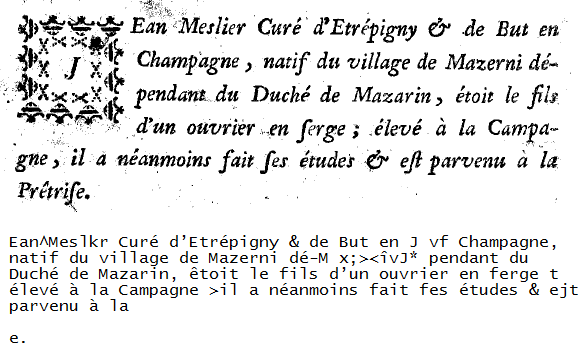
\includegraphics[scale=1]{3-Methode-CREA/images/1-pre-traitement-semantique/exemple_probleme_OCR.png}
}
\caption{Exemple d'un cas difficile pour un logiciel de reconnaissance optique de caractères (extrait du Testament de Jean Meslier - 1762)}
\label{figure:3-I-3-NettoyageDonnees-ProblemeOCR}
\end{figure}

\hspace{0pt}
\vfill

%\newpage
\bigskip


\begin{table}[ht]
\centering
\begin{tabular}{| l | l |}
\hline
\textbf{Conservées} 				& \textbf{Supprimées} \\
\hline
abréviation ($ABR$) 					& adverbe ($ADV$) \\ \hline
adjectif ($ADJ$)  						& article ($DET{:}ART$) \\ \hline
interjection ($INT$) 					& pronom possessif ($DET{:}POS$) \\ \hline
nom propre et mots inconnus ($NAM$) 	& conjonction ($KON$) \\ \hline
nom commun ($NOM$)						& pronom ($PRO$) \\ \hline
numéro ($NUM$)							& pronom démonstratif ($PRO{:}DEM$) \\ \hline
préposition ($PRP$)						& pronom indéfini ($PRO{:}IND$) \\ \hline
ponctuation ($PUN$)						& pronom personnel ($PRO{:}PER$) \\ \hline
ponctuation de citation ($PUN{:}cit$)	& pronom possessif ($PRO{:}POS$) \\ \hline
point final ($SENT$)					& pronom relatif ($PRO{:}REL$) \\ \hline
symbole ($SYM$)							& préposition plus article ($PRP{:}det$) \\ \hline
verbe - conditionnel ($VER{:}cond$)		& \\ \hline
verbe - futur ($VER{:}futu$)			& \\ \hline
verbe - impératif ($VER{:}impe$)		& \\ \hline
verbe - imparfait ($VER{:}impf$)		& \\ \hline
verbe - infinitif ($VER{:}infi$)		& \\ \hline
verbe - participe passé ($VER{:}pper$)	& \\ \hline
verbe - participe présent ($VER{:}ppre$)		& \\ \hline
verbe - présent ($VER{:}pres$)					& \\ \hline
verbe - passé simple ($VER{:}simp$)				& \\ \hline
verbe - imparfait du subjonctif ($VER{:}subi$)	& \\ \hline
verbe - présent subjonctif ($VER{:}subp$)		& \\ \hline
\end{tabular}
\caption{Classes grammaticales conservées ou supprimées}
\label{table:3-I-3-NettoyageDonnees-Classesgrammaticales}
\end{table}




%%%%%%%%%%%%%%%%%%%%%%%%%%%%%%%%%%%%%%%%%%%%
\clearpage % Clean for pictures and tables %
\newpage   % Clean for pictures and tables %
%%%%%%%%%%%%%%%%%%%%%%%%%%%%%%%%%%%%%%%%%%%%

\subsection{Désambiguïsation (PI.3)}
\label{subsection:CREA:PI.4-Desambiguisation}

La \textit{désambiguïsation} est l'étape clé du pré-traitement sémantique.
En effet, la phase suivante d'analyse structurelle manipulant des documents et les termes communs entre ces documents, il est nécessaire de standardiser ces termes en retrouvant les concepts (au sens du triangle sémiotique~\cite{zargayouna2015recherche}) qui leurs sont attachés.
Cette étape permet donc à la fois de désambiguïser les termes selon le contexte, mais aussi de les lier à un concept particulier.
Ainsi, les problèmes de polysémie\footnote{\og \textit{La plupart [des mots] sont polysémiques, c'est-à-dire pourvus de plusieurs sens} \fg~\cite{goosse2016bon} } et de synonymie\footnote{\og \textit{Les synonymes sont des mots qui, appartenant à la même classe grammaticale, ont à peu près la même signification} \fg~\cite{goosse2016bon} } sont résolus grâce au contexte du document.

À l'issue de cette étape, une liste de termes désambiguïsés avec l'identifiant unique de concept associé est fournie.

\bigskip

Nous avons implémenté cette étape avec BabelFy~\cite{moro2014entity}\cite{moro2014multilingual}, un outil de désambiguïsation et d'annotation sémantique, lié à BabelNet~\cite{navigli2012babelnet}, un réseau sémantique multilingue manipulant des concepts et des entités nommées lié à WordNet~\cite{miller1995wordnet} et Wikipedia.
BabelFy est capable de déduire quel entité nommée ou concept est manipulé pour chacun des termes, et ce dans une multitude de langues.
Son autre atout réside dans son lien avec BabelNet, et donc l'encyclopédie Wikipedia : les concepts et entités de la vie courante (technologies, produits commerciaux, ...) sont reconnaissables dans les textes, y compris lorsque ceux-ci sont spécifiques à un domaine bien particulier.
BabelFy cherche donc les liens les plus probables entre un terme et un concept ou une entité nommée, puis il indique l'identifiant unique retenu et différents scores liés à ses traitements.

\bigskip

La figure~\ref{figure:3-I-4-Desambiguisation-BabelFyGUI} illustre parfaitement l'utilité de BabelFy par rapport à d'autres outils plus traditionnels concernant les termes particuliers à certains domaines.
On peut voir dans le formulaire d'entrée que le terme \og \textit{PHP} \fg est reconnu par le navigateur web, mais pas \og \textit{MySQLi} \fg (le correcteur orthographique intégré le faisant remarquer).
Cependant, grâce à son accès à une base de connaissances suffisamment large, BabelFy arrive à reconnaître l'extension peu connue des non-initiés qu'est \og \textit{MySQLi} \fg .
Dans le cadre de cours d'informatique, tous les termes clés sont donc automatiquement extraits des supports de cours insérés, en plus d'être identifiés de façon unique.


%\begin{figure*} % Figure flottante
\begin{figure}[ht]
\centering
%\includegraphics[width=3in]{images/VerySmallModels_text.png}
%%\includegraphics[scale=0.6]{images/VerySmallModels_text.png}
\centerline{  % FORCE FIGURE OUTSIDE THE MARGIN !!! BUT STILL CENTERING !!!
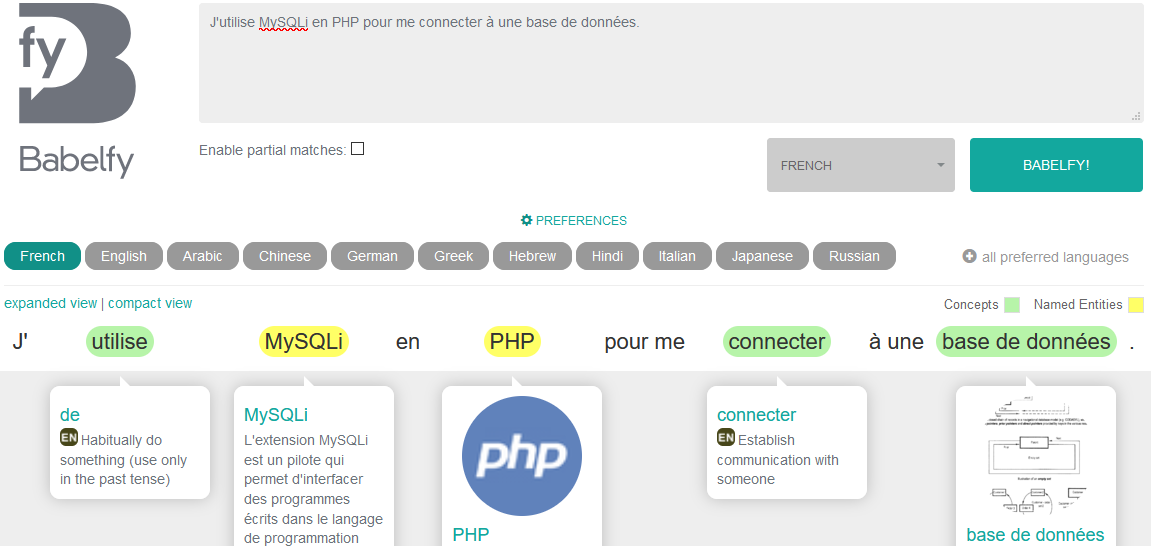
\includegraphics[scale=0.54]{3-Methode-CREA/images/1-pre-traitement-semantique/desambiguisation-GUI.png}
}
\caption{Exemple de désambiguïsation et d'annotation sémantique avec BabelFy}
\label{figure:3-I-4-Desambiguisation-BabelFyGUI}
\end{figure}
%\end{figure*} % Figure flottante
% To use it : fig~\ref{label}

\bigskip

Parmi les choix de paramétrage de BabelFy, nous avons opté pour des correspondances exactes (\textit{MatchingType.EXACT\_MATCHING}) et les candidats obtenant les meilleurs scores (\textit{ScoredCandidates.TOP}), afin d'obtenir les sens dont BabelFy est le plus sûr.
BabelFy n'autorisant pas des textes de plus de $ 10.000 $ caractères, les textes transmis sont équitablement découpés pour distribuer autant que possible le plus de caractères dans le moins de groupes possibles, tout en respectant la limite et en conservant entiers les mots aux extrémités.
L'intérêt de transmettre de grands groupes de mots est que le contexte est mieux compris par BabelFy, et donc la qualité de ses résultats en est améliorée.
L'essentiel étant d'éviter l'utilisation d'une simple division euclidienne qui ne transmettrait que dans un seul cas des groupes parfaitement égaux, et inversement, dans beaucoup d'autres cas le dernier groupe serait relativement petit.


%%%%%%%%%%%%%%%%%%%%%%%%%%%%%%%%%%%%%%%%%%%%
%\clearpage % Clean for pictures and tables %
%\newpage   % Clean for pictures and tables %
%%%%%%%%%%%%%%%%%%%%%%%%%%%%%%%%%%%%%%%%%%%%

\bigskip

\subsection{Filtrage des termes (PI.4)}
\label{subsection:CREA:PI.5-FiltrageTermes}

La dernière étape, le \textit{filtrage des termes}, consiste à améliorer la qualité des listes de termes désambiguïsés en supprimant les termes hors sujet.
L'intérêt est de ne proposer à l'utilisateur que des termes en lien avec le domaine, et donc de produire des fragments contenant des termes pertinents pour le cas géré.
BabelFy met à disposition plusieurs scores suite à ses traitements.
Le score de cohérence mesure en particulier la connectivité d'un terme avec les autres termes du texte transmis~\cite{prohaska2017masterthesis} (d'où l'intérêt d'envoyer les plus grands groupes de mots possibles de façon équitable).

\bigskip

% É
Nous avons empiriquement constaté que beaucoup de termes inutiles pouvaient être facilement éliminés en fixant un score minimum de cohérence à atteindre.
Le score de cohérence correspond au niveau de connectivité du terme désambiguïsé par rapport aux autres termes du même texte fourni à BabelFy.
Les termes dont le score de cohérence est strictement supérieur à $ 0,05 $ sont conservés.
Ce score élimine malgré tout quelques occurrences de termes intéressants, mais celles-ci restent relativement faibles par rapport à la quantité de termes hors sujet.

\bigskip

À l'issue de cette étape nous obtenons pour chaque document une liste de termes désambiguïsés et en lien avec le sujet.
Ces listes sont fusionnées sous forme de matrice d'occurrences, afin d'obtenir un format utile pour la phase suivante.

Étant donné que plusieurs documents peuvent contenir les mêmes termes désambiguïsés, on crée une matrice rassemblant les occurrences des termes contenus dans chaque document.
La figure~\ref{figure:3-I-5-MatriceOccurrences} illustre une matrice d'occurrences où l'on peut voir dix documents d'entrée (Cours 1 à 10) et quatre termes (web, php, sql, mysql) avec leurs identifiants dans la base de connaissances BabelNet.
On peut voir en pratique que le terme \og \textit{php} \fg, dont l'identifiant unique est \og $bn{:}01753580n$ \fg, apparait \textit{15} fois dans le \textit{Cours 1} et \textit{53} fois dans le \textit{Cours 2}.
Cette matrice est un pré-requis pour la phase suivante appliquant l'ACF.

%\begin{figure*} % Figure flottante
\begin{figure}[ht]
\centering
%\includegraphics[width=3in]{images/VerySmallModels_text.png}
%%\includegraphics[scale=0.6]{images/VerySmallModels_text.png}
\centerline{  % FORCE FIGURE OUTSIDE THE MARGIN !!! BUT STILL CENTERING !!!
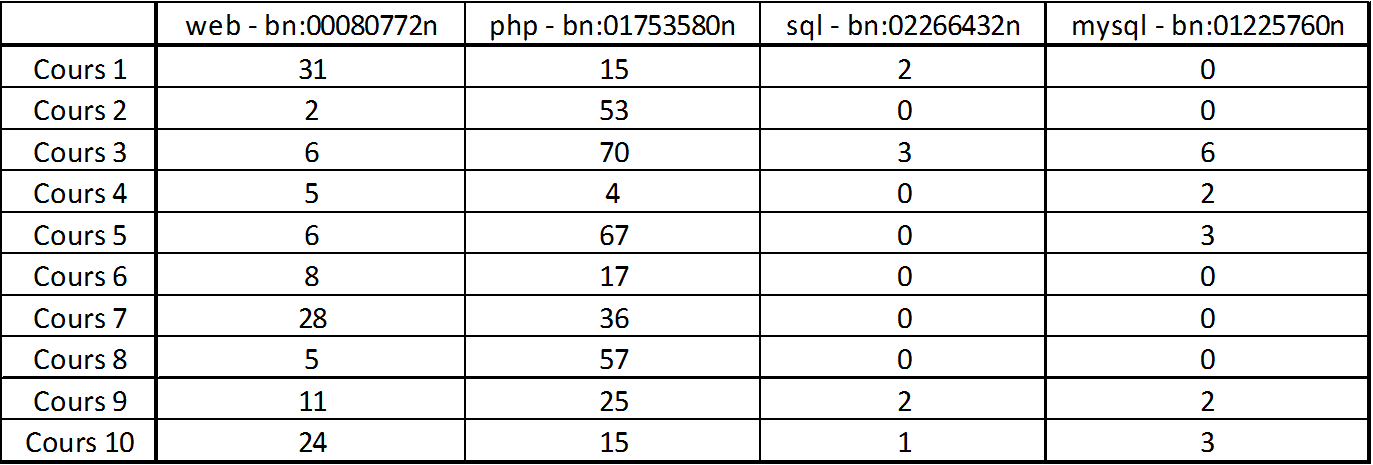
\includegraphics[scale=0.85]{3-Methode-CREA/images/1-pre-traitement-semantique/exemple_matrice_occurrences.png}
}
\caption{Exemple de matrice d'occurrences}
\label{figure:3-I-5-MatriceOccurrences}
\end{figure}
%\end{figure*} % Figure flottante
% To use it : fig~\ref{label}




%%%%%%%%%%%%%%%%%%%%%%%%%%%%%%%%%%%%%%%%%%%%%%%%%%%%%%%%%%%%%%%%%%%%%%%%%%%%%%%%%%%%%%%%%%
%%%%%%%%%%%%%%%%%%%%%%%%%%%%%%%%%%%%%%%%%%%%%%%%%%%%%%%%%%%%%%%%%%%%%%%%%%%%%%%%%%%%%%%%%%
%%%%%%%%%%%%%%%%%%%%%%%%%%%%%%%%%%%%%%%%%%%%%%%%%%%%%%%%%%%%%%%%%%%%%%%%%%%%%%%%%%%%%%%%%%
%%%%%%%%%%%%%%%%%%%%%%%%%%%%%%%%%%%%%%%%%%%%%%%%%%%%%%%%%%%%%%%%%%%%%%%%%%%%%%%%%%%%%%%%%%
%%%%%%%%%%%%%%%%%%%%%%%%%%%%%%%%%%%%%%%%%%%%%%%%%%%%%%%%%%%%%%%%%%%%%%%%%%%%%%%%%%%%%%%%%%
%%%%%%%%%%%%%%%%%%%%%%%%%%%%%%%%%%%%%%%%%%%%%%%%%%%%%%%%%%%%%%%%%%%%%%%%%%%%%%%%%%%%%%%%%%

%%%%%%%%%%%%%%%%%%%%%%%%%%%%%%%%%%%%%%%%%%%%
\clearpage % Clean for pictures and tables %
\newpage   % Clean for pictures and tables %
%%%%%%%%%%%%%%%%%%%%%%%%%%%%%%%%%%%%%%%%%%%%

%%%%%%%%%%%%%%%%%%%%%%%%%%%%%%%%%%%%%%%%%%%%%%%%%%%%%%%%%%%%%%%%%%%%%%%%%%%%%%%%%%%%%%%%%%
%%%%%%%%%%%%%%%%%%%%%%%%%%%%%%%%%%%%%%%%%%%%%%%%%%%%%%%%%%%%%%%%%%%%%%%%%%%%%%%%%%%%%%%%%%
%%%%%%%%%%%%%%%%%%%%%%%%%%%%%%%%%%%%%%%%%%%%%%%%%%%%%%%%%%%%%%%%%%%%%%%%%%%%%%%%%%%%%%%%%%
%%%%%%%%%%%%%%%%%%%%%%%%%%%%%%%%%%%%%%%%%%%%%%%%%%%%%%%%%%%%%%%%%%%%%%%%%%%%%%%%%%%%%%%%%%
%%%%%%%%%%%%%%%%%%%%%%%%%%%%%%%%%%%%%%%%%%%%%%%%%%%%%%%%%%%%%%%%%%%%%%%%%%%%%%%%%%%%%%%%%%
%%%%%%%%%%%%%%%%%%%%%%%%%%%%%%%%%%%%%%%%%%%%%%%%%%%%%%%%%%%%%%%%%%%%%%%%%%%%%%%%%%%%%%%%%%

\section{Analyse structurelle : métriques de qualité et extraction des clusters}
\label{subsection:CREA:PII-AnalyseStructurelle}

La deuxième phase (PII) de la méthode CREA, l'analyse structurelle, a pour objectif d'extraire des clusters de termes en identifiant les relations entre les termes et documents traités lors de la phase précédente.
Lors de la création des documents, des connaissances ont été mobilisées afin d'organiser de manière intelligible (connaissances tacites) des notions à transmettre (connaissances explicites) à d'autres individus.
Pour le domaine de l'enseignement, il s'agit d'identifier les liens entre les notions abordées dans les supports de cours afin de réorganiser ces notions sous forme d'un syllabus, ou plus concrètement, sous forme de clusters de termes.
Cette phase se déroule en trois étapes successives illustrées par la figure~\ref{figure:3-II-AnalyseStructurelle}.


%\begin{figure*} % Figure flottante
\begin{figure}[ht]
\centering
%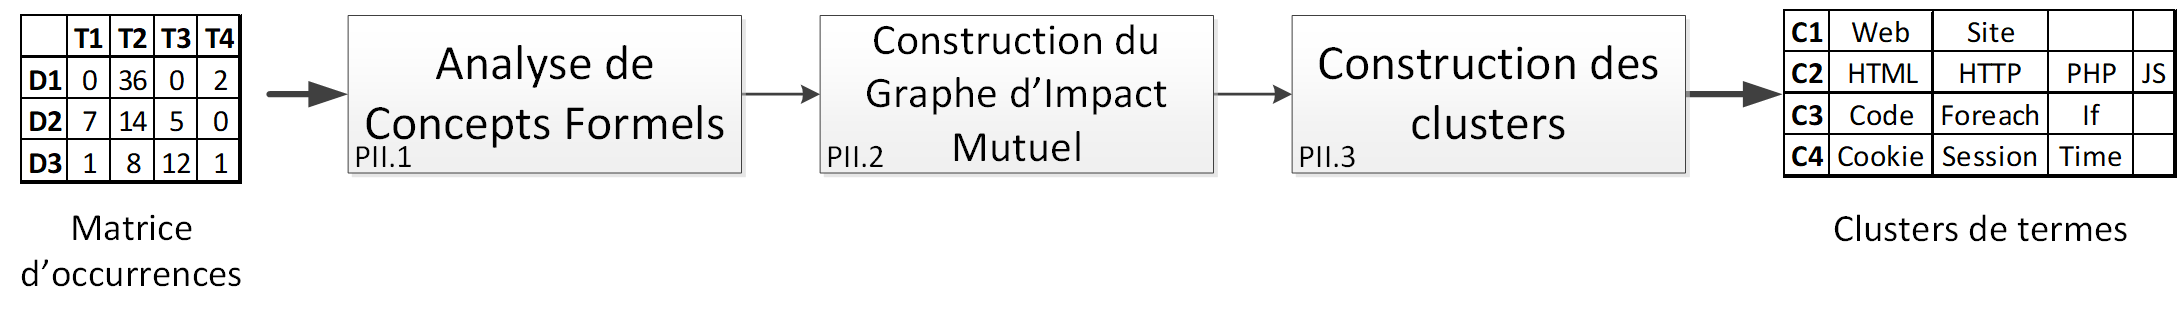
\includegraphics[scale=0.6]{3-Methode-CREA/images/schema_analyse_structurelle.png}
\centerline{  % FORCE FIGURE OUTSIDE THE MARGIN !!! BUT STILL CENTERING !!!
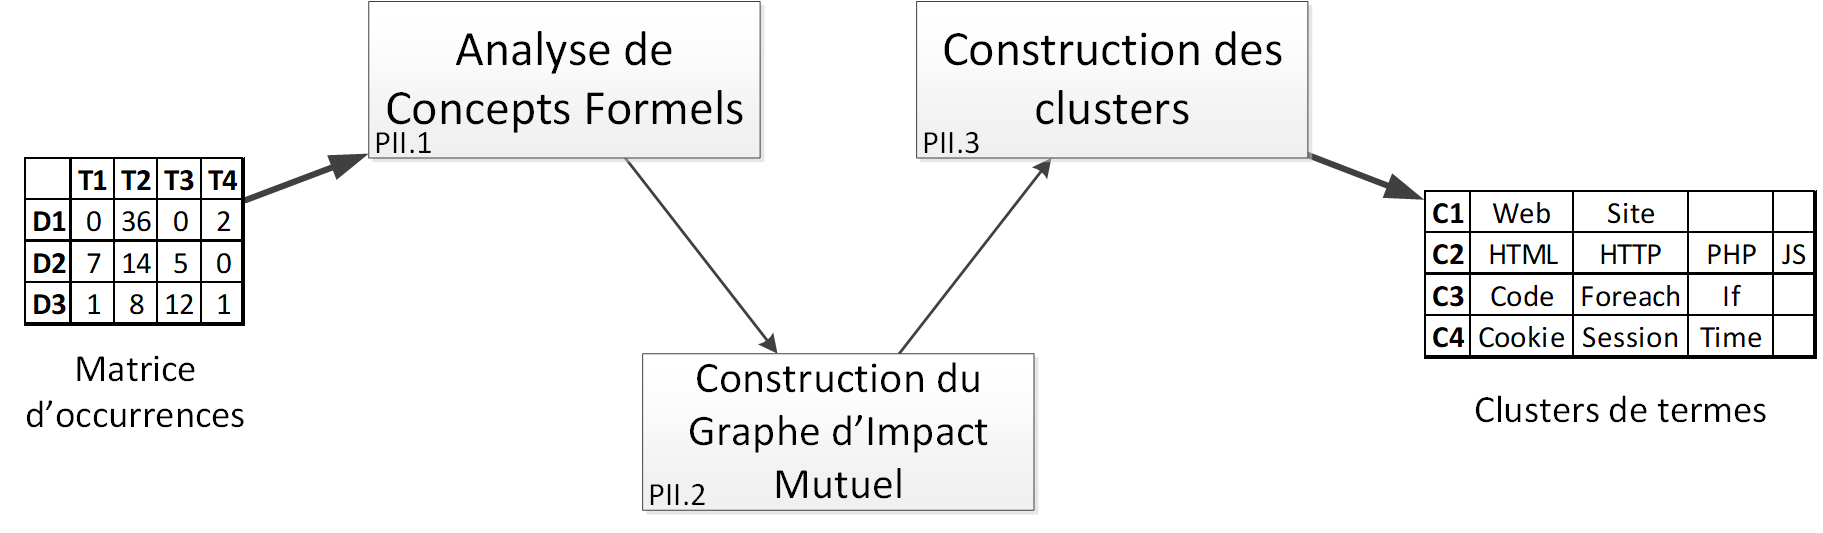
\includegraphics[scale=0.6]{3-Methode-CREA/images/schema_analyse_structurelle_ESCALIER.png}
}
\caption{Les étapes de la phase d'analyse structurelle}
\label{figure:3-II-AnalyseStructurelle}
\end{figure}
%\end{figure*} % Figure flottante
% To use it : fig~\ref{label}

\begin{itemize}
\item Analyse de Concepts Formels (PII.1) : Les techniques d'analyse de concepts formels servent à analyser les liens entre les termes et les documents les contenant afin de calculer deux métriques (l'impact mutuel et la similarité conceptuelle). Ces métriques nous permettent d'évaluer la pertinence des documents entre eux à partir des termes les plus fréquents, mais aussi d'établir la similarité des termes entre eux.
\item Construction du Graphe d'Impact Mutuel (PII.2) : L'impact mutuel entre les termes et les documents est représenté graphiquement afin de mesurer la pertinence des documents entre eux tout en affichant un ensemble de termes explicitant les principaux sujets abordés dans ces documents. Cette métrique permet d'indiquer quels documents devraient être retirés pour obtenir les meilleurs regroupements de termes.
\item Construction des clusters (PII.3) : À partir de la similarité conceptuelle des termes entre eux, des clusters de termes sont formés pour présenter à l'utilisateur les fragments réutilisables pour le cas traité.
\end{itemize}


\subsection{Analyse de Concepts Formels (PII.1)}
\label{subsection:CREA:PII.1-ACF}

L'Analyse de Concepts Formels, présentée en sous-section~\ref{subsection:Contexte:TechniquesUtilisees:ACF}, est un ensemble de techniques permettant de \og \textit{découvrir et [de] structurer des connaissances} \fg~\cite{jaffal2019aide} à partir d'une matrice rassemblant des \textit{objets} et leurs \textit{attributs}.
Appliquée au domaine de l'enseignement, avec une matrice de supports de cours et de termes les composant, il s'agit de rechercher les relations entre ces termes et les supports de cours afin d'en extraire des métriques de similarité conceptuelle et d'impact mutuel.
Ces métriques permettent ensuite d'obtenir une vision globale de l'ensemble du corpus documentaire, et d'en déduire les sujets centraux à partir des termes, mais également la pertinence des supports de cours par rapport à ces sujets centraux.
Le principe général de l'ACF se déroule en plusieurs sous-étapes illustrées par la figure~\ref{figure:3-II-1-ACF-Details}.

%\begin{figure*} % Figure flottante
\begin{figure}[ht]
\centering
%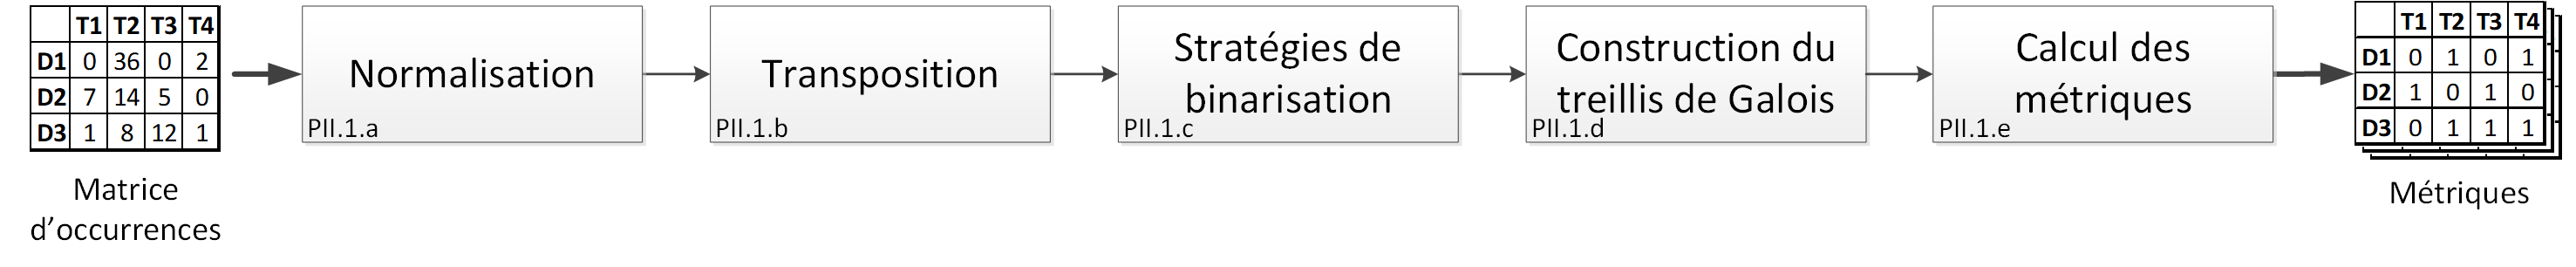
\includegraphics[scale=0.49]{3-Methode-CREA/images/schema_analyse_structurelle-ACF.png}
\centerline{  % FORCE FIGURE OUTSIDE THE MARGIN !!! BUT STILL CENTERING !!!
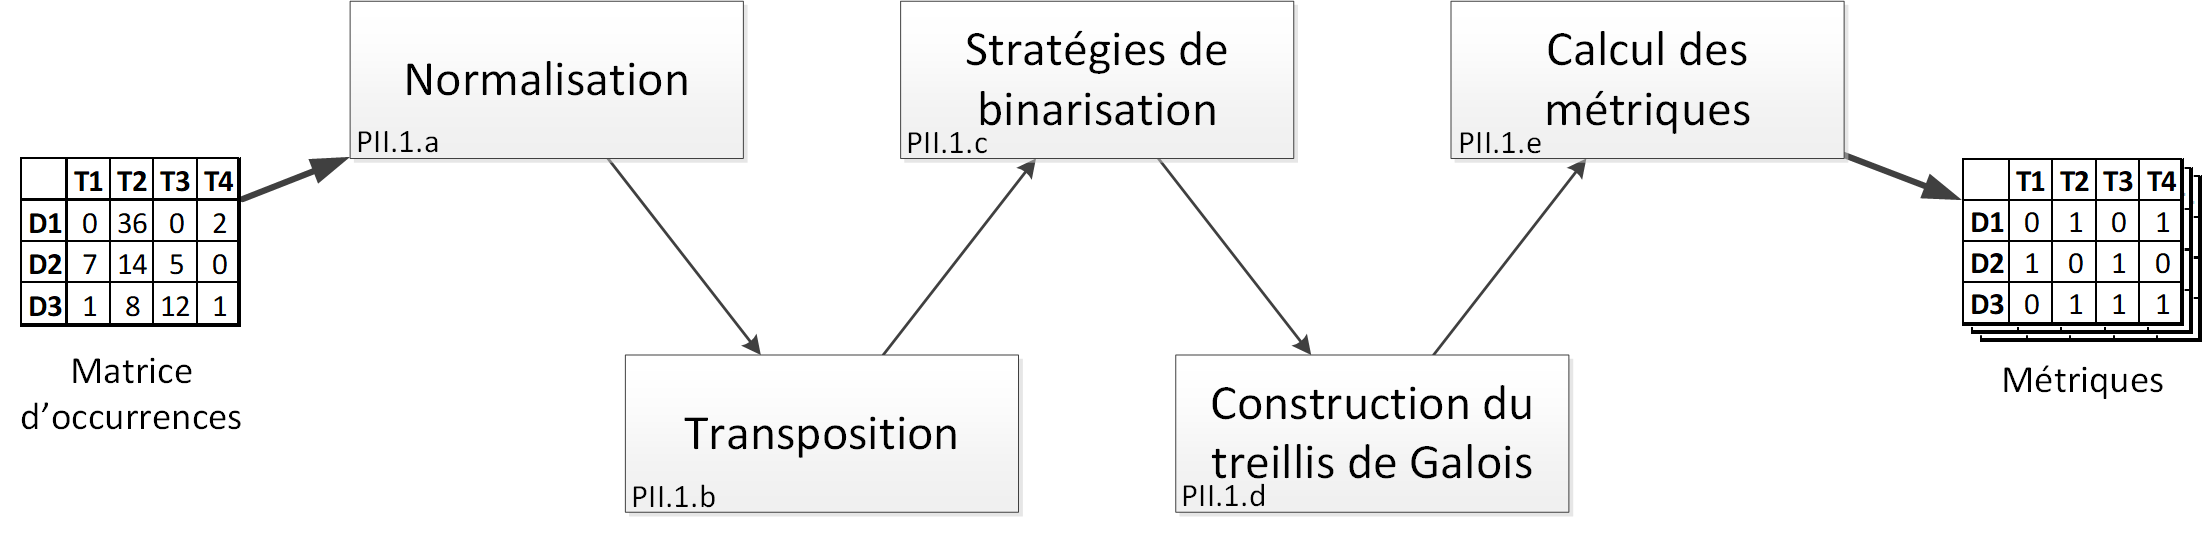
\includegraphics[scale=0.55]{3-Methode-CREA/images/schema_analyse_structurelle-ACF_ESCALIER.png}
}
\caption{Les sous-étapes de l'analyse de concepts formels}
\label{figure:3-II-1-ACF-Details}
\end{figure}
%\end{figure*} % Figure flottante
% To use it : fig~\ref{label}


\subsubsection{Normalisation (PII.1.a) :}
\label{subsubsection:CREA:PII.1.a-normalisation}

Afin de binariser la matrice d'occurrences pour en faire un \textit{contexte formel}  nous avons choisi de prendre en compte la taille des documents.
Un document contenant des milliers de termes au milieu de documents contenant une centaine de termes chacun créera une disproportion.
Afin de limiter l'effet de ce biais, une première étape vise à normaliser les quantités proportionnellement à la taille des documents : les occurrences des termes sont transformées en proportions d'occurrences dans chacun des documents.
La figure~\ref{figure:3-II-1-a-Normalisation} illustre l'étape de normalisation.

%\begin{figure*} % Figure flottante
\begin{figure}[ht]
\centering
%\includegraphics[width=3in]{images/VerySmallModels_text.png}
%%\includegraphics[scale=0.6]{images/VerySmallModels_text.png}
\centerline{  % FORCE FIGURE OUTSIDE THE MARGIN !!! BUT STILL CENTERING !!!
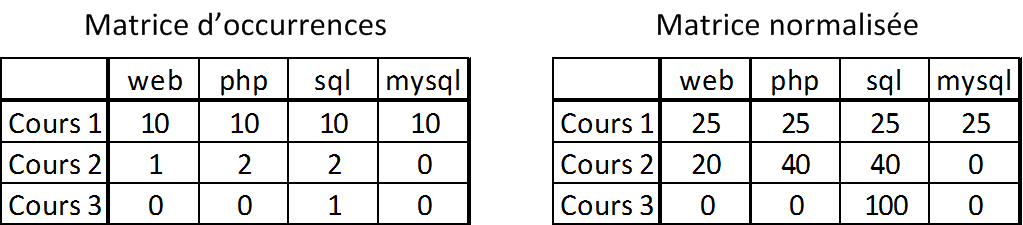
\includegraphics[scale=1]{3-Methode-CREA/images/2-analyse-structurelle/exemple_normalisation.png}
}
\caption{Exemple de normalisation d'une matrice d'occurrences}
\label{figure:3-II-1-a-Normalisation}
\end{figure}
%\end{figure*} % Figure flottante
% To use it : fig~\ref{label}

%
%XX;T1;T2;T3;T4
%C1;01;00;42;01
%C2;10;10;10;10
%C3;01;02;02;00
%C4;00;00;01;00
%
%XX;T1;T2;T3;T4
%C1;03;00;96;03
%C2;25;25;25;25
%C3;20;40;40;00
%C4;00;00;100;0
%


\subsubsection{Transposition (PII.1.b) :}
\label{subsubsection:CREA:PII.1.b-transposition}

Le sens de lecture des lignes et colonnes de la matrice est important pour les stratégies de binarisation, l'ACF, et l'interprétation des fragments qui en seront extraits.
L'ACF construisant un treillis avec des \textit{objets} caractérisés par des \textit{attributs} issus d'un \textit{contexte formel} (une matrice binaire), et les stratégies se basant sur ces caractéristiques pour générer ce \textit{contexte formel}, il est important que la matrice d'entrée soit correctement présentée : les \textit{objets} forment les lignes, et les \textit{attributs} forment les colonnes.
En l'état, les documents (objets) sont caractérisés par les termes (attributs) les composant.
Afin de changer de point de vue, et mettre en avant les connaissances réutilisables, c'est-à-dire les liens entre termes et documents, il est nécessaire de transposer la matrice pour permettre de caractériser les termes (objets) selon les documents (attributs) dans lesquels ils apparaissent.
La figure~\ref{figure:3-II-1-b-Transposition} illustre l'étape de transposition.

%\begin{figure*} % Figure flottante
\begin{figure}[ht]
\centering
%\includegraphics[width=3in]{images/VerySmallModels_text.png}
%%\includegraphics[scale=0.6]{images/VerySmallModels_text.png}
\centerline{  % FORCE FIGURE OUTSIDE THE MARGIN !!! BUT STILL CENTERING !!!
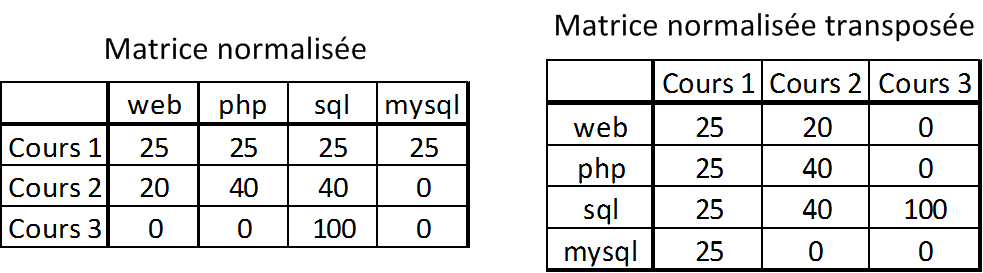
\includegraphics[scale=1]{3-Methode-CREA/images/2-analyse-structurelle/exemple_transposition.png}
}
\caption{Exemple de transposition pour caractériser les termes selon les documents où ils apparaissent}
\label{figure:3-II-1-b-Transposition}
\end{figure}
%\end{figure*} % Figure flottante
% To use it : fig~\ref{label}


\subsubsection{Stratégies de binarisation (PII.1.c) :}
\label{subsubsection:CREA:PII.1.c-strategies}

La matrice d'occurrences étant normalisée et transposée pour mettre en avant les termes caractérisés par les documents dans lesquels ils apparaissent, il est maintenant possible d'appliquer une stratégie permettant de transformer les occurrences en valeurs binaires pour obtenir un \textit{contexte formel} nécessaire à la construction du treillis dans les étapes suivantes.
Une stratégie de binarisation définit un algorithme qui transforme les valeurs d'une matrice de l'intervalle $ [ 0, +\infty [ $ vers la paire $ \{ 0, 1 \} $.

\bigskip

Il existe actuellement plusieurs stratégies~\cite{jaffal2015refinement}\cite{jaffal2019aide} pour permettre à l'ACF de présenter différentes informations contenues dans une matrice multivaluée.
Ces stratégies sont présentées en sous-section~\ref{subsubsection:Contexte:ACF-StrategiesBinarisation}.
Les métriques visées par la méthode CREA impliquent de générer les contextes formels de plusieurs de ces stratégies.
La stratégie \textit{directe} permet d'avoir une vision d'ensemble du corpus utile pour évaluer l'ensemble des sujets centraux et la pertinence des documents entre eux (les valeurs non-nulles sont remplacées par des 1, et les valeurs nulles sont remplacées par des 0).
La stratégie \textit{haute} utilisant un $ \beta = 1.00 $ permet de ne retenir que les termes dont les valeurs de fréquences d'apparition dans les documents sont les plus hautes.
Cette stratégie permet de retenir les termes les plus fréquents pour l'ensemble du corpus, mais également pour certains ensemble de documents.

\bigskip

La figure~\ref{figure:3-II-1-c-Strategies-Exemple-Directe-Haute} illustre ces deux stratégies (Directe et Haute avec un $ \beta $ fixé à 1,00).
On remarque que les valeurs non nulles de chaque ligne sont distribuées différemment entre les deux stratégies : \textit{sql} apparaissant dans tous les cours de façon non négligeable à chaque fois, c'est-à-dire que tous les cours parlent de \textit{sql} et l'un lui est dédié, il est le seul terme à être conservé sur la stratégie haute.
Cet exemple, plutôt extrême, sert à bien distinguer les objectifs différents des deux stratégies : la stratégie directe permet de voir que le cours \textit{C3} ne dispose que d'une seule notion, et devrait donc être retiré du corpus, à l'inverse, la stratégie haute récupère en effet le sujet central de \textbf{l'ensemble} du corpus documentaire, qui est \textit{sql}.
Un enseignant doit donc s'assurer tout d'abord avec la stratégie directe que les documents insérés sont cohérents, puis, une fois les documents correctement sélectionnés, il peut appliquer la stratégie haute pour en extraire les notions essentielles.


%\begin{figure*} % Figure flottante
\begin{figure}[ht]
\centering
%\includegraphics[width=3in]{images/VerySmallModels_text.png}
%%\includegraphics[scale=0.6]{images/VerySmallModels_text.png}
\centerline{  % FORCE FIGURE OUTSIDE THE MARGIN !!! BUT STILL CENTERING !!!
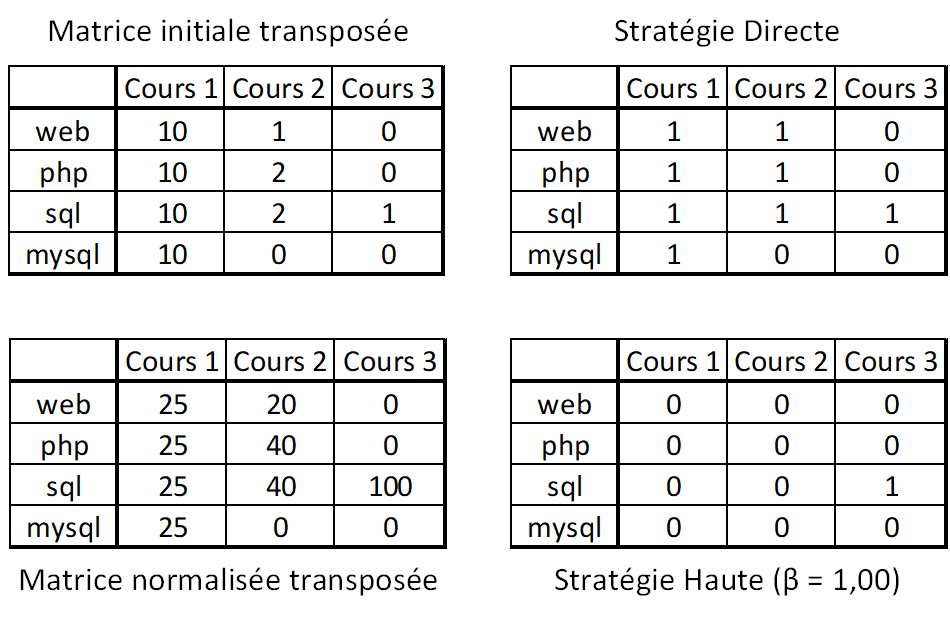
\includegraphics[scale=1]{3-Methode-CREA/images/2-analyse-structurelle/exemple_strategies_directe_haute_beta=1.00.png}
}
\caption{Exemple d'application des stratégies directe et haute avec un $ \beta = 1,00 $}
\label{figure:3-II-1-c-Strategies-Exemple-Directe-Haute}
\end{figure}
%\end{figure*} % Figure flottante
% To use it : fig~\ref{label}



\subsubsection{Construction du treillis de Galois (PII.1.d) :}
\label{subsubsection:CREA:PII.1.d-treillis}

Le \textit{contexte formel} généré avec les stratégies de binarisation contient maintenant des termes liés à des documents par des $ 0 $ et des $ 1 $.
Il peut donc être transformé en un \textit{treillis de Galois} composé de \textit{concepts formels} qui serviront à produire l'impact mutuel et la similarité conceptuelle.
Le \textit{treillis} est un graphe dont chaque n\oe{}ud correspond à un \textit{concept formel}.
Chaque \textit{concept formel} rassemble des \textit{objets} et leurs \textit{attributs} (et inversement, des \textit{attributs} et les \textit{objets} auxquels ils sont rattachés).
Dans notre cas, il s'agit donc de créer des concepts formels contenant des termes et les documents où ils apparaissent.
La construction d'un treillis est présentée plus en détails en sous-section~\ref{subsubsection:Contexte:ACF-ConstructionTreillis}.

Nous avons utilisé la bibliothèque \textit{Concepts}\footnote{ \href{https://concepts.readthedocs.io/en/stable/}{Page du projet \textit{Concepts} pour Python} } en Python pour automatiser la construction des treillis à partir des matrices précédentes.


\subsubsection{Calcul des métriques du treillis (PII.1.e) :}
\label{subsubsection:CREA:PII.1.e-metriquestreillis}

L'ACF permet de calculer l'impact mutuel et la similarité conceptuelle sur le treillis généré~\cite{jaffal2019aide}.
Ces métriques sont présentées en sous-section~\ref{subsubsection:Contexte:ACF-MetriquesTreillis}.
Dans le cas de la méthode CREA, nous nous concentrons particulièrement sur l'impact mutuel, qui permet de générer des graphiques utiles pour l'amélioration de la qualité des données, et la similarité conceptuelle permettant la construction des clusters de termes.


\paragraph{Similarité Conceptuelle entre objets :}
\label{mystep:CREA:PII.1.e-metrique-similariteobjets}

La \textit{similarité conceptuelle} permet de comparer deux objets (respectivement attributs) en tenant compte de leur présence dans l'ensemble du treillis.
C'est-à-dire, est-ce que les deux objets apparaissent souvent ensemble dans les concepts formels ?
Pour un enseignant, cette métrique permet de retrouver quelles notions sont les plus similaires entre elles pour les regrouper.
Techniquement, dans le cadre de la méthode CREA, la matrice de similarité conceptuelle permet d'établir la similarité entre l'ensemble des termes afin de pouvoir créer des clusters.
Suite à nos expérimentations (présentées dans la sous-section~\ref{subsubsection:Evaluation:ProtocoleEvaluation:ValidationsStructurellesFonctionnellesREX:Structurelle}), nous avons fixé les paramètres de cette métrique en utilisant le treillis représentant la matrice de stratégie haute avec un $ \beta = 1.00 $ .
En effet, nous avons empiriquement constaté que la stratégie haute permet d'obtenir les termes les plus représentatifs de l'ensemble des documents, donc d'établir une vue globale des notions abordées, et $ \beta = 1.00 $ filtre suffisamment les termes pour obtenir les meilleurs résultats.



\paragraph{Impact mutuel entre un objet et un attribut :}
\label{mystep:CREA:PII.1.e-metrique-impactmutuel}

L'\textit{impact mutuel} analyse la "\textit{force de la relation entre un objet et un attribut en fonction des concepts formels qui les associent}"~\cite{jaffal2019aide}.
Cette métrique permet de visualiser quels documents partagent le plus de notions, et réciproquement, quelles notions sont les plus présentes dans les documents.
Pour un enseignant, il s'agit d'identifier les notions clés de l'ensemble du corpus documentaire, mais aussi quels documents sont les moins représentatifs (afin de les retirer).
En assemblant les mesures d'impact mutuel entre tous les objets et attributs, une \textit{matrice d'impact mutuel} est formée.
Cette matrice d'impact mutuel permet de générer un \textit{graphe d'impact mutuel} dans l'étape suivante.
Afin d'avoir une vision d'ensemble, elle est générée à partir du treillis représentant la matrice de stratégie directe.


\subsection{Construction du Graphe d'Impact Mutuel (PII.2)}
\label{subsection:CREA:PII.2-GrapheImpactMutuel}

La \textit{Construction du Graphe d'Impact Mutuel} permet de visualiser la matrice d'impact mutuel et en déduire plusieurs informations importantes pour l'utilisateur.
Le graphe d'impact mutuel a la particularité d'être bi-parti, en proposant des n\oe{}uds de la classe des objets, et des n\oe{}uds de la classe des attributs.
Dans la méthode CREA, il s'agit donc de n\oe{}uds représentant des termes et des documents.

\bigskip

Une communauté de termes qui apparaissent visuellement au centre du graphe permet d'identifier clairement les termes les plus employés dans l'ensemble du corpus.
Cet ensemble central est déduit du degré de connexion des n\oe{}uds de la classe des termes : plus le n\oe{}ud d'un terme est connecté à des n\oe{}uds de cours, plus il est situé au centre (et réciproquement, moins il est connecté, plus il est éloigné).
À partir de cette visualisation, il est possible de comprendre quels sujets sont abordés par l'ensemble des documents, ou au contraire par certains documents précis.
La visualisation permet également de voir si quelques documents sont complètement ou partiellement hors sujet : les documents hors sujet étant peu reliés aux termes apparaissant dans l'ensemble central, leurs n\oe{}uds sont particulièrement excentrés.

\bigskip

Pour notre usage, l'utilisateur peut donc déduire si le corpus documentaire correspond à ses attentes selon les notions abordées (via les termes au centre), et éventuellement si certains documents devraient être retirés dans le cas où ceux-ci sont partiellement ou complètement hors sujet.

\bigskip

Lors de nos expérimentations, nous avons utilisé le logiciel \textit{Gephi}~\cite{bastian2009gephi} pour visualiser les matrices d'impact mutuel sous forme de graphe.
Précisément, nous avons utilisé la spatialisation \textit{Force Atlas} qui est un algorithme basé sur les forces~\cite{venturini2021we} (\og \textit{force-based} \fg ou encore \og \textit{force-directed} \fg en anglais).

La \textit{visualisation} cherche à projeter sur un plan des graphiques de points et de lignes~\cite{venturini2021we} (\og \textit{points-and-lines charts} \fg en anglais).
La \textit{spatialisation} est une forme de visualisation qui s'intéresse particulièrement à l'espace créé par la projection des données : l'espace de sortie n'est plus considéré comme une contrainte (réduisant le nombre de dimensions), mais bien comme une donnée de sortie liée aux objets projetés.
Les algorithmes basés sur les forces permettent de placer les n\oe{}uds d'un graphe en respectant un principe : les n\oe{}euds se repoussent mutuellement avec une \textit{force de répulsion}, et les arcs attirent les n\oe{}uds avec une \textit{force d'attraction}~\cite{venturini2021we}.
Ces algorithmes tendent à espacer les n\oe{}uds faiblement liés, et au contraire, à rapprocher les n\oe{}uds fortement liés~\cite{venturini2021we}.
L'algorithme \textit{Force Atlas} est une spatialisation propre à Gephi dont l'objectif est de \og \textit{permettre une interprétation rigoureuse des graphes [...] le plus directement et lisiblement possible malgré un temps d'exécution assez long} \fg~\cite{gephi2016spatialisationFR}.
Il peut s'appliquer sur des graphes comptant de $ 1 $ à $ 10000 $ n\oe{}uds avec une complexité en $ O(N^2) $~\cite{gephi2011tutoriallayout}\cite{gephi2016spatialisationFR}.
\textit{Force Atlas} permet à l'utilisateur de sélectionner plusieurs paramètres tels que les forces d'attraction, de répulsion, et quelques autres afin de placer les n\oe{}uds~\cite{jacomy2014forceatlas2}.
%
% Sources de Force Atlas :
% https://github.com/gephi/gephi/blob/db454c59cc9da3f47b7268de4ccbfa73b7f5245e/modules/LayoutPlugin/src/main/java/org/gephi/layout/plugin/forceAtlas/ForceAtlasLayout.java#L64
%


La figure~\ref{figure:3-II-2-Graphe-zoom} illustre le graphe d'impact mutuel entre des termes et des documents.
Sur la gauche, le graphe dans son ensemble est affiché.
Sur la droite, un zoom est effectué sur les termes apparaissant au c\oe{}ur du graphe.
Les n\oe{}uds en rouge sont les termes connectés à tous les cours, les n\oe{}uds en orange sont connectés à tous les cours sauf 1, les n\oe{}uds en jaune sont connectés à tous les cours sauf 2, et ainsi de suite.
Les n\oe{}uds gris représentent les supports de cours.
En lisant ce graphe, on peut voir que les termes qui apparaissent au c\oe{}ur du graphe sont \textit{post}, \textit{méthode post}, \textit{nombre}, \textit{langage}, \textit{donnée}, \textit{fichier}, \textit{code}, \textit{php}, \textit{navigateur}, \textit{site}.
La combinaison de certains termes permet de comprendre assez vite qu'il s'agit de cours sur du développement web, en particulier de PHP.


La figure~\ref{figure:3-II-2-Graphe-cours} illustre cette fois la distance entre les documents.
Typiquement, le cours \textit{C6} semble très éloigné de l'ensemble, tout comme le cours \textit{C3}, et légèrement \textit{C5}.
Il apparait donc judicieux de se pencher plus en détails sur ces derniers pour vérifier leur pertinence pour le corpus documentaire rassemblé.



Au delà du manque de pertinence d'un document par rapport aux termes, un utilisateur peut également décider d'écarter un document si certains termes contenus ne devraient pas apparaître dans les clusters finaux.
À l'issue de cette étape, l'utilisateur peut donc décider de supprimer certains documents et ré-exécuter l'analyse de concepts formels à partir de la matrice épurée des documents en question, ou de continuer avec les données déjà générées.


% esthétique
\newpage

%\vfill
%\hspace{0pt}

\begin{figure}[ht!]
\centering
\centerline{  % FORCE FIGURE OUTSIDE THE MARGIN !!! BUT STILL CENTERING !!!
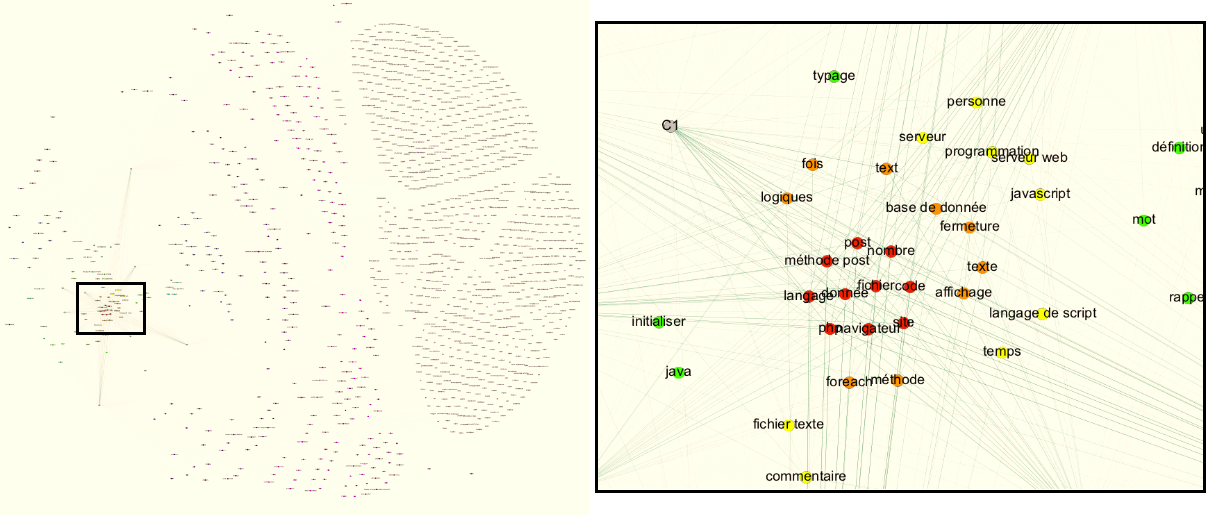
\includegraphics[scale=0.6]{3-Methode-CREA/images/2-analyse-structurelle/exemple_graphe.png}
}
\caption{Graphe d'impact mutuel (généré avec Gephi en utilisant la spatialisation \textit{Force Atlas} et la coloration par \textit{partition} selon le \textit{degré})}
\label{figure:3-II-2-Graphe-zoom}
\end{figure}


\begin{figure}[ht!]
\centering
\centerline{  % FORCE FIGURE OUTSIDE THE MARGIN !!! BUT STILL CENTERING !!!
%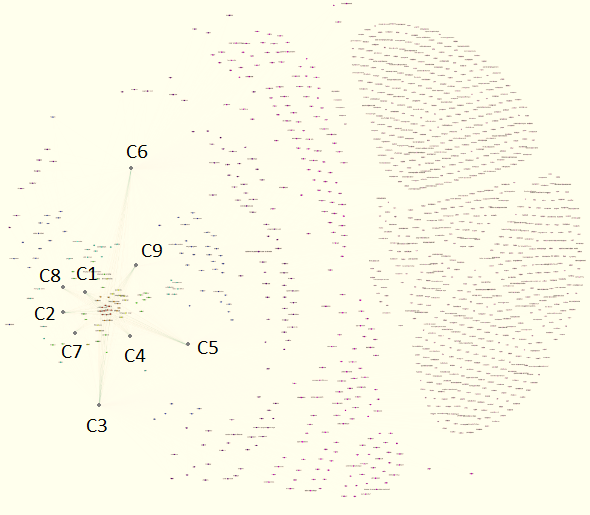
\includegraphics[scale=0.2]{3-Methode-CREA/images/2-analyse-structurelle/exemple_graphe_large_cours.png}
% 0.7
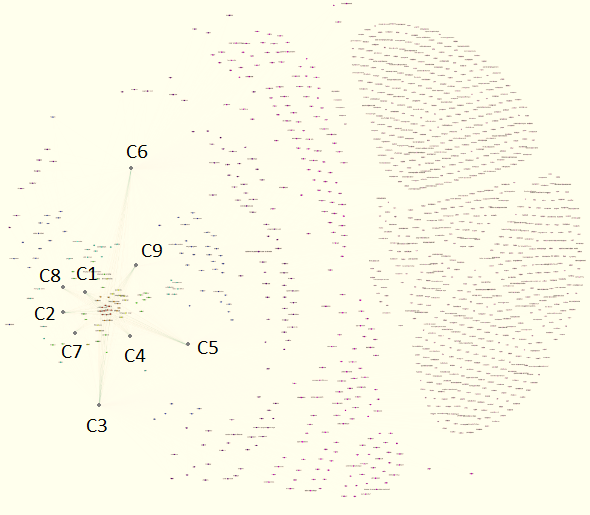
\includegraphics[scale=0.78]{3-Methode-CREA/images/2-analyse-structurelle/exemple_graphe_large_cours.png}
}
\caption{Graphe d'impact mutuel (généré avec Gephi en utilisant la spatialisation \textit{Force Atlas} et la coloration par \textit{partition} selon le \textit{degré})}
\label{figure:3-II-2-Graphe-cours}
\end{figure}


%\hspace{0pt}
%\vfill

% esthétique
\clearpage

\subsection{Construction des clusters (PII.3)}
\label{subsection:CREA:PII.3-ConstructionClusters}

La \textit{construction des clusters} est l'ultime étape construisant des clusters à partir de la matrice de similarité conceptuelle des termes.
Ces clusters correspondent aux fragments réutilisables, c'est-à-dire dans le contexte de l'enseignement, les notions à aborder ensemble et pouvant former un syllabus.
Plusieurs techniques de clustering sont présentées en sous-section~\ref{subsection:Contexte:TechniquesUtilisees:Clustering}.
Selon l'implémentation employée, il est parfois nécessaire de transformer la matrice de similarité en une \textit{matrice de dissimilarité}.

\bigskip

Dans nos travaux, nous avons opté pour la \textit{classification ascendante hiérarchique} (ou CAH) afin d'obtenir des clusters non-recouvrants permettant de ne placer chaque terme que dans un seul cluster, tout en indiquant le nombre de clusters que l'utilisateur souhaite.
En pratique, l'implémentation de CAH inclue dans la bibliothèque SciPy~\cite{2020SciPy-NMeth} en Python exige une matrice de distance ou à minima une matrice avec la dissimilarité entre chacun des objets.
Ainsi, pour transformer notre matrice de similarité en matrice de dissimilarité (composée de valeurs entre $ 0 $ et $ 1 $), nous avons utilisé la méthode la plus simple présentée dans~\cite{rakotomalala2020pratique} consistant à soustraire chaque valeur de similarité à la valeur de similarité maximale, c'est-à-dire soustraire chacune des valeurs à $ 1 $ (les $ 1 $ devenant des $ 0 $, et ainsi de suite jusqu'aux $ 0 $ devenant des $ 1 $).
La formule~\eqref{equation:3-Calcul-Dissimilarite} illustre ce calcul.

\begin{equation}
\text{\textit{dissimilarité}}(\text{\textit{objet A}}, \text{\textit{objet B}}) = 1 - \text{\textit{similarité}}(\text{\textit{objet A}}, \text{\textit{objet B}})
\label{equation:3-Calcul-Dissimilarite}
\end{equation}


\bigskip

Afin d'appliquer la CAH, nous avons utilisé les bibliothèques scikit-learn~\cite{scikit-learn} et SciPy~\cite{2020SciPy-NMeth}.
Précisément, nous avons appliqué trois traitements successifs afin de générer les clusters finaux.
\begin{enumerate}
\item Nous standardisons tout d'abord les valeurs grâce à \textit{sklearn.preprocessing.scale()} en laissant les paramètres par défaut.
\item Nous appliquons ensuite le traitement effectuant l'agglomération des clusters individuels avec \textit{scipy.cluster.hierarchy.linkage()}.
Nous demandons l'usage de la méthode de Ward (\texttt{\textit{method='ward'}}) avec une métrique euclidienne pour ce traitement. (\texttt{\textit{metric='euclidean'}})
\item Nous utilisons enfin \textit{scipy.cluster.hierarchy.fcluster()} pour récupérer la liste des clusters.
Nous demandons de rechercher un maximum de clusters possibles \\ (\texttt{\textit{criterion='maxclust'}}) en visant 8 clusters (\texttt{\textit{t=8}}).
\end{enumerate}

\bigskip

La figure~\ref{figure:3-II-3-Clusters} illustre un résultat en huit clusters, c'est-à-dire pour huit séances.
Les clusters n'étant pas ordonnés, c'est à l'enseignant que revient ce choix.
Une technique d'ordonnancement temporelle, encore en cours d'évaluation, est proposée en sous-section~\ref{subsection:Conclusion:PerspectivesAmeliorations:AnalyseTemporelle}.

\bigskip

Dans tous les cas, ces clusters constituent une base réutilisable de termes dont l'utilisateur peut se servir pour traiter son nouveau cas.


\bigskip

\vfill
\hspace{0pt}

%\begin{figure*} % Figure flottante
\begin{figure}[ht]
\centering
\centerline{  % FORCE FIGURE OUTSIDE THE MARGIN !!! BUT STILL CENTERING !!!
% 0.65
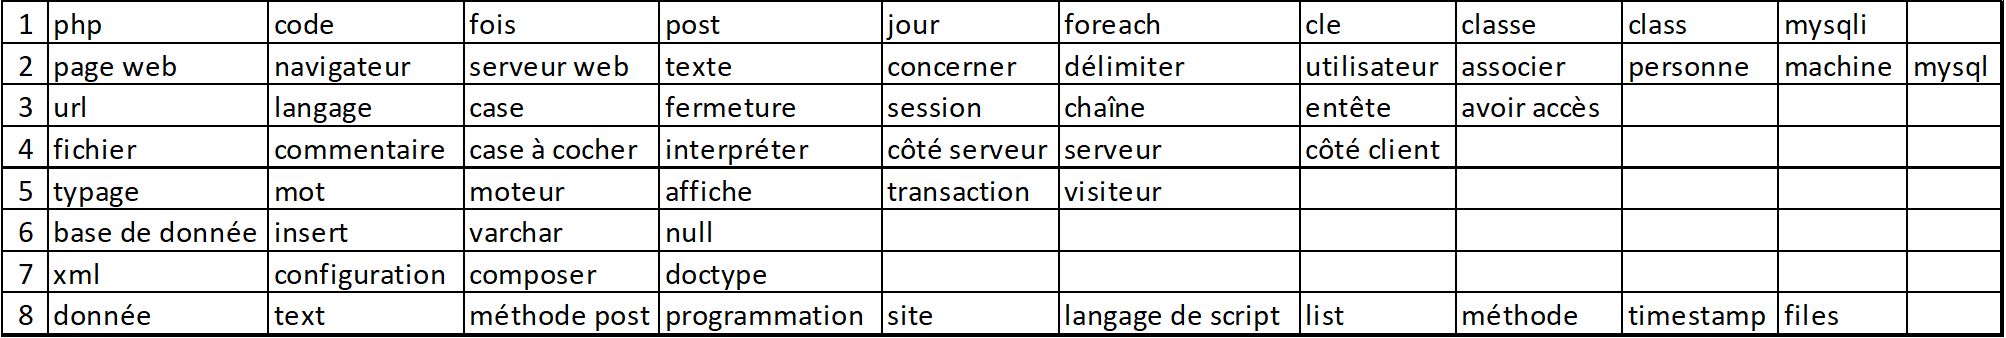
\includegraphics[scale=0.68]{3-Methode-CREA/exemples/clusters/clusters.png}
}
\caption{Liste de huit clusters générés}
\label{figure:3-II-3-Clusters}
\end{figure}
%\end{figure*} % Figure flottante
% To use it : fig~\ref{label}


\hspace{0pt}
\vfill



%%%%%%%%%%%%%%%%%%%%%%%%%%%%%%%%%%%%%%%%%%%%%%%%%%%%%%%%%%%%%%%%%%%%%%%%%%%%%%%%%%%%%%%%%%
%%%%%%%%%%%%%%%%%%%%%%%%%%%%%%%%%%%%%%%%%%%%%%%%%%%%%%%%%%%%%%%%%%%%%%%%%%%%%%%%%%%%%%%%%%
%%%%%%%%%%%%%%%%%%%%%%%%%%%%%%%%%%%%%%%%%%%%%%%%%%%%%%%%%%%%%%%%%%%%%%%%%%%%%%%%%%%%%%%%%%
%%%%%%%%%%%%%%%%%%%%%%%%%%%%%%%%%%%%%%%%%%%%%%%%%%%%%%%%%%%%%%%%%%%%%%%%%%%%%%%%%%%%%%%%%%
%%%%%%%%%%%%%%%%%%%%%%%%%%%%%%%%%%%%%%%%%%%%%%%%%%%%%%%%%%%%%%%%%%%%%%%%%%%%%%%%%%%%%%%%%%
%%%%%%%%%%%%%%%%%%%%%%%%%%%%%%%%%%%%%%%%%%%%%%%%%%%%%%%%%%%%%%%%%%%%%%%%%%%%%%%%%%%%%%%%%%
%
%\newpage
%
%%%%%%%%%%%%%%%%%%%%%%%%%%%%%%%%%%%%%%%%%%%%%%%%%%%%%%%%%%%%%%%%%%%%%%%%%%%%%%%%%%%%%%%%%%
%%%%%%%%%%%%%%%%%%%%%%%%%%%%%%%%%%%%%%%%%%%%%%%%%%%%%%%%%%%%%%%%%%%%%%%%%%%%%%%%%%%%%%%%%%
%%%%%%%%%%%%%%%%%%%%%%%%%%%%%%%%%%%%%%%%%%%%%%%%%%%%%%%%%%%%%%%%%%%%%%%%%%%%%%%%%%%%%%%%%%
%%%%%%%%%%%%%%%%%%%%%%%%%%%%%%%%%%%%%%%%%%%%%%%%%%%%%%%%%%%%%%%%%%%%%%%%%%%%%%%%%%%%%%%%%%
%%%%%%%%%%%%%%%%%%%%%%%%%%%%%%%%%%%%%%%%%%%%%%%%%%%%%%%%%%%%%%%%%%%%%%%%%%%%%%%%%%%%%%%%%%
%%%%%%%%%%%%%%%%%%%%%%%%%%%%%%%%%%%%%%%%%%%%%%%%%%%%%%%%%%%%%%%%%%%%%%%%%%%%%%%%%%%%%%%%%%


%%%%%%%%%%%%%%%%%%%%%%%%%%%%%%%%%%%%%%%
%\section{Analyse temporelle : organisation des scénarios}% :
%\label{section:CREA:PIII-AnalyseTemporelle}
%
%
%\subsection{Découpage des documents en sections (PIII.1)}
%\label{subsection:CREA:PIII.1-DecoupageDocuments}
%
%\subsection{Sélection des étiquettes temporelles (PIII.2)}
%\label{subsection:CREA:PIII.2-SelectionEtiquettesTemporelles}
%
%\subsection{Étiquetage temporel des clusters (PIII.3)}
%\label{subsection:CREA:PIII.3-EtiquetageTemporelClusters}
%
%\subsection{Organisation en séances (PIII.4)}
%\label{subsection:CREA:PIII.4-OrganisationSeances}
